%%%%%%%%%%%%%%%%%%%%%%%%%%%%%%%%%%%%%%%%%%%%%%%%%%%%%%%%%%%%%%%%%%%%%%%%%%%%%%%%%%%%%%%%%%%%%%%%%%%%
%%                                  Dissertação - Latex
%%
%%      UNICAMP - Faculdade de Engenharia Mecânica
%%      Gilberto Luis Valente da Costa
%%      2012
%%
%%%%%%%%%%%%%%%%%%%%%%%%%%%%%%%%%%%%%%%%%%%%%%%%%%%%%%%%%%%%%%%%%%%%%%%%%%%%%%%%%%%%%%%%%%%%%%%%%%%%


% Classe do documento
%   Para a opção {book}, se o documento possui margem direita 2cm e esquerda 3cm, com esta opcao, as
% margens serao alternadas - folhas pares com margem direita 2cm e esquerda 3cm e folhas ımpares com
% margem direita 3cm e esquerda 2cm
\documentclass[12pt,twoside]{report}

% Pacotes e comandos customizados
%%%%%%%%%%%%%%%%%%%%%%%%%%%%%%%%%%%%%%%%%%%%%%%%%%%%%%%%%%%%%%%%%%%%%%%%%%%%%%%%%%%%%%%%%%%%%%%%%%%%
%%                                    Configuração do Latex
%%
%%      UNICAMP - Faculdade de Engenharia Mecânica
%%      Gilberto Luis Valente da Costa
%%      2012
%%
%%%%%%%%%%%%%%%%%%%%%%%%%%%%%%%%%%%%%%%%%%%%%%%%%%%%%%%%%%%%%%%%%%%%%%%%%%%%%%%%%%%%%%%%%%%%%%%%%%%%


%===================================================================================================
%                                      PACOTES PRINCIPAIS
%===================================================================================================
%% Codificação e formatação básica do LaTeX
% Dimensoes da pagina
\usepackage[top=3cm,left=3cm,right=2cm,bottom=3cm]{geometry}    % Dimensões da página
\usepackage[portuges, brazilian]{babel} % Hiphenação em portugues
\usepackage[utf8]{inputenc}             % Codificação do arquivo
\usepackage[T1]{fontenc}
\usepackage{times}                      % Pacote de fonte Times
\usepackage{lhelp}                      % Denine macros úteis
\usepackage{ccaption}                   % Opções para capítulos
\usepackage{indentfirst}                % Identação do primeiro parágrafo
\usepackage{fancyhdr}                   % Controlar os cabeçalhos e rodapés
\usepackage{enumerate}                  % Para usar enumerações
\usepackage{cmap}                       % Mapear caracteres especiais no PDF

\usepackage{floatflt}                   % Quebra de texto em figuras e tabelas
\usepackage{colortbl}                   % Adicionar cor às tabelas
\usepackage{fancyvrb}                   % Texto verbatim sofisticado
\usepackage{wrapfig}                    % Produz figuras que o texto pode ficar ao redor
\usepackage{url}                        % Adiciona URLs
\usepackage{multirow}                   % Permite construir células multi-linhas

% Essencial para colocar funções e outros símbolos matemáticos
\usepackage{amsmath, amssymb, amsthm}
\usepackage{amscd, amsfonts, textcomp}
\usepackage{psfrag,layout}

%% Links dinâmicos
%% Suporte para hipertexto, links para referências e figuras
%% To Dvi.
%\usepackage[dvipdfmx,plainpages=false,pdfpagelabels,colorlinks=true,
%citecolor=black,linkcolor=black,urlcolor=black,filecolor=black,
%bookmarksopen=true]{hyperref}
% To pdflatex
\usepackage[pdftex, plainpages=false, pdfpagelabels, colorlinks=true,
citecolor=black,linkcolor=black, urlcolor=black, filecolor=black,
bookmarksopen=true]{hyperref}

\usepackage[dvipsnames,svgnames,table]{xcolor}
\usepackage{pdfpages}			% Inclui paginas em pdf no arquivo
\usepackage{epstopdf}			% Converte figuras em formato eps para pdf
\usepackage{color}			% Suporte para cores
\usepackage{transparent}		% Suporte para vários conjuntos de cores
\usepackage{siunitx}			% Sistema internacional de unidades
\usepackage{lipsum}

\usepackage[all]{hypcap}                % Soluciona o problema com o hyperref e capítulos
\usepackage{wasysym}                    % Símbolos especiais com \female e \male etc.
\usepackage{bigstrut}                   % Espaçamento na tabela
\usepackage{comment}                    % Comentar várias linhas simultâneas
\usepackage{epigraph}                   % Epígrafe
\usepackage[titles,subfigure]{tocloft}  % Permite formatar o sumário
\usepackage{makeidx}
\usepackage{emptypage}			 % Retira o número de páginas em branco
\usepackage{afterpage}
\usepackage{kantlipsum}			 % mock text

\usepackage{setspace}                   % Para definir espaçamento entre as linhas
\usepackage{listings}                   % Para Inserir código fonte
%===================================================================================================


%===================================================================================================
%                                       ELEMENTOS GRÁFICOS
%===================================================================================================
\usepackage{graphics}                   % Suporte padrão para gráficos
\usepackage{graphicx}                   % Suporte avançado para gráficos
\usepackage[]{graphicx}                 % Para incluir figuras (pacote extendido)
\usepackage[normalsize]{subfigure}      % Possibilita a utilização de subfiguras
% \usepackage{subfig}                     % Criar figura dividida em subfiguras
\usepackage{epsfig}                     % Uso de figuras eps.
\usepackage{epsf}

% Caso queira guardar as figuras em uma pasta separada
% (descomente e) defina o caminho para o diretório:
%\graphicspath{{./figuras/}}
\usepackage{caption}                    % Customizar as legendas de figuras e tabelas
\usepackage{multicol}                   % Criar ambientes com 2 ou mais colunas
%===================================================================================================


%===================================================================================================
%===================================================================================================
%% Tabelas
\usepackage{array}                      % Elementos extras para formatação de tabelas
\usepackage{booktabs}                   % Tabelas com qualidade de publicação
\usepackage{longtable}                  % Para criar tabelas maiores que uma página
\usepackage{lscape}                     % adicionar tabelas e figuras como landscape

%% Lista de Abreviações
% \usepackage[notintoc,portuguese]{nomencl}   % Cria lista de abreviações
\usepackage{nomencl}
\makenomenclature

% %  Lista de Tabela de siglas e simbolos.
%\usepackage{tabela-simbolos} 
% %  Letras maiúsculas são colocados antes dos símbolos de minúsculas.
%\usepackage[caixa=Mm]{tabela-simbolos}
% %  Define a ordem em que vai aparecer os simbolos, as letras gregas e romanas.
%\usepackage[romanos=2,gregos=3,simbolos=1]{tabela-simbolos}

%% Notas de rodapé
\usepackage{footnote}                   % Lidar com notas de rodapé em diversas situações
\makesavenoteenv{tabular}               % Notas criadas nas tabelas ficam no fim das tabelas
\usepackage{pifont}                     % Acesso a PostScript Symbol padrão e fontes Dingbats
\usepackage{lastpage}                   % Conta o número de páginas
\usepackage{ifoddpage}			 % Incluinde páginas impares.
\newcommand\alwaysodd[1]{%
  \checkoddpage
  \ifoddpage
    #1%
  \else
    \mbox{}\clearpage#1%
  \fi
}
% \usepackage{ifthen,changepage}


%% Referências bibliográficas e afins
\usepackage[round]{natbib}              % Citações tipo (nome-ano)
%\usepackage{natbib}                    % Citações tipo [nome-ano]

% Adicionar bibliografia, índice e conteúdo na Tabela de conteúdo
% Não inclui lista de tabelas e figuras no índice
\usepackage[nottoc,notlof,notlot]{tocbibind}

%% Pontuação e unidades
\usepackage{icomma}		% Posicionar inteligentemente a vírgula como separador decimal
\usepackage[tight]{units}	% Formatar as unidades com as distâncias corretas
%===================================================================================================


%===================================================================================================
%                                   FORMATAÇÕES DE TEXTO
%===================================================================================================
\special{papersize=215.9mm,279.4mm}     % Tamanho do papel (neste caso papel carta)
\pagenumbering{roman}                   % Numeração das paginas iniciais em romano
\setlength{\parindent}{1cm}             % Parágrafo de 1cm
% \setlength{\mathindent}{1cm}          % Indentação das fórmulas matemáticas
\setlength{\fboxsep}{1mm}               %   Espaçamento do texto para o frame, também define
                                        % espaçamento entre colunas da tabela
\frenchspacing                          % Não põe um espaço adicional após ponto final
\sloppy                                 % Força que todas as linhas fiquem dentro das margens
\raggedbottom                           % Para não permitir espaços extra no texto
\def\figurename{Figura.}                % Define como a palavra figura será escrito
\def\tablename{Tabela.}                 % Define como a palavra tabela será escrito

\newcommand{\eq}[1]{Equação~(\ref{#1})}	% Facilita a citação de Equações
\newcommand{\figu}[1]{Figura~\ref{#1}}		% Facilita a citação de Figuras
\newcommand{\tab}[1]{Tabela~\ref{#1}}		% Facilita a citação de Tabelas


% Citação tipo (AUTOR, ano), conforme ABNT
\renewcommand{\cite}[1]{(\textsc{\citeauthor{#1}},~\citeyear{#1})}
%
\theoremstyle{definition}
\newtheorem{defi}{Definição}[chapter]		% Para introduzir uma definição
\newtheorem{teo}{Teorema}[chapter]		% Para introduzir um teorema
\newcommand{\nomunit}[1]{%
\renewcommand{\nomentryend}{\dotfill[#1]}}	% Colocar unidades na lista de Abreviaturas e siglas

%% Estes comandos criam os subgrupos na Lista de Abreviaturas e Siglas
\renewcommand{\nomgroup}[1]{%
  \ifthenelse{\equal{#1}{A}}{\item[\textbf{Letras Latinas}]}{\hrulefill%			a
    \ifthenelse{\equal{#1}{C}}{\item[\textbf{Letras Gregas}]}}}}				c
        \ifthenelse{\equal{#1}{G}}{\item[\textbf{Subscritos}]}}}}}}			e
           \ifthenelse{\equal{#1}{K}}{\item[\textbf{Siglas}]}{}}{}}{}}{}}{}}{}}%		f
%
\setcounter{secnumdepth}{5}	% Serve pra introduzir um quinto nível de seções (subsubsubsection)
\setcounter{tocdepth}{5}	% Serve pra introduzir um quinto nível de seções (subsubsubsection)
%
\makeatletter			% Changes the category code of '@' character to 11
%===================================================================================================


%===================================================================================================
%                                      PARA INSERIR CÓDIGO FONTE
%===================================================================================================
\lstset{
  numbers=left,
  stepnumber=1,
  firstnumber=1,
  numberstyle=\tiny,
  extendedchars=true,
  breaklines=true,
  frame=tb,
  basicstyle=\footnotesize,
  stringstyle=\ttfamily,
  showstringspaces=false
}
\renewcommand{\lstlistingname}{Código}
\renewcommand{\lstlistlistingname}{Lista de Listagens}
%===================================================================================================


%===================================================================================================
%                                          OPERADORES
%===================================================================================================
% Conforme a necessidade de cada trabalho
\newcommand{\vectornorm}[1]{\left|\left|#1\right|\right|}   % Facilita a introdução da norma ||w||
\newcommand{\argmax}{\operatornamewithlimits{argmax}}       % Facilita a escrita de argmax
\newcommand{\latex}{\LaTeX~}                                % Facilita a escrita de LaTeX
\newlength\figureheight
\newlength\figurewidth
%==================================================================================================


%===================================================================================================
%                             FORMATANDO SEÇÕES, TABELAS E EQUAÇÕES
%===================================================================================================
\@addtoreset{figure}{chapter}
\renewcommand{\thefigure}{\thechapter.\@arabic\c@figure}

\@addtoreset{equation}{chapter}
\renewcommand{\theequation}{\thechapter.\@arabic\c@equation}

\@addtoreset{table}{chapter}
\renewcommand{\thetable}{\thechapter.\@arabic\c@table}

\def\chapter{\@startsection{chapter}{1}
          {\z@}{12pt minus 0pt}{12pt minus 0pt}{\renewcommand{\rmdefault}{phv}\large\bf}}
\def\appendix{\@startsection{chapter}{1}
          {\z@}{12pt minus 0pt}{12pt minus 0pt}
          {\large{\textsf{\textbf{APÊNDICE}}}~~\renewcommand{\rmdefault}{phv}\large\bf}}
\def\section{\@startsection{section}{2}
          {\z@}{12pt minus 0pt}{12pt minus 0pt}{\renewcommand{\rmdefault}{phv}\bf}}
\def\subsection{\@startsection{subsection}{3}
          {\z@}{12pt minus 0pt}{12pt minus 0pt}{\renewcommand{\rmdefault}{phv}\bf}}
\def\subsubsection{\@startsection{subsubsection}{4}
          {\z@}{12pt minus 0pt}{12pt minus 0pt}{\renewcommand{\rmdefault}{phv}\bf}}
\def\subsubsubsection{\@startsection{subsubsubsection}{5}
          {\z@}{12pt minus 0pt}{12pt minus 0pt}{\renewcommand{\rmdefault}{phv}\bf}}
         
\newcounter {anexo}[chapter]
\def\anexo{\@startsection{chapter}{1}
          {\z@}{12pt minus 0pt}{12pt minus 0pt}
	  {\large{\textsf{\textbf{ANEXO}}}~~\renewcommand{\rmdefault}{phv}\large\bf}}
%===================================================================================================


%===================================================================================================
%                                         SUB-SUB-SUB-SECTION
%===================================================================================================
\newcounter {subsubsubsection}[subsubsection]
\renewcommand\thesubsubsubsection{}
% \newcommand\subsubsubsection{\@startsection{subsubsubsection}{4}{\z@}%
%                             {12pt minus 0pt}{12pt minus 0pt}{\normalfont\normalsize\it}}
% Espaçamento do numero da subsubsubseção em relação à marge no sumário.
\newcommand*\l@subsubsubsection{\@dottedtocline{3}{8em}{2.2em}}
\newcommand*{\subsubsubsectionmark}[1]{}

%---------------------------------------------------------------------------------------------------

\def\thechapter{\arabic{chapter}}
\def\thesection{\thechapter.\arabic{section}}	
\def\thesubsection{\thesection.\arabic{subsection}}
% \def\thesubsubsection{\Alph{subsubsection}}
\def\thesubsubsection{}
\makeatother				% Reverts (\makealetter) this to its original catcode of 12.

%\renewcommand\cftsecfont{\bf}                % Títulos das seções em negrito no sumário
%\renewcommand{\cftsecleader}{\cftdotfill{\cftnodots}}  % Elimina os pontos na frente das seções no sumário
%\setlength\cftbeforesecskip{12pt}            % Espaçamento antes da seção no sumário
%\renewcommand{\cftsecindent}{0 em}           % Espaçamento do numero da seção em relação à marge no sumário
%\renewcommand{\cftsecnumwidth}{1.9 em}       % Espaçamento do título da seção em relação ao número no sumário
%\renewcommand{\cftsubsecindent}{1.9 em}      % Espaçamento do numero da subseção em relação à marge no sumário
%\renewcommand{\cftsubsecnumwidth}{2.8 em}    % Espaçamento do título da subseção em relação ao número no sumário
%\renewcommand{\cftsubsubsecindent}{4.7 em}   % Espaçamento do numero da subsubseção em relação à marge no sumário
\renewcommand{\cftsubsubsecnumwidth}{1.9 em}  %     Espaçamento do título da subsubseção em relação
                                              % ao número no sumário
%===================================================================================================


%===================================================================================================
%                               FORMATAÇÃO DAS REFERÊNCIAS BIBLIOGRÁFICAS
%===================================================================================================
\renewcommand\refname{}
\makeatletter
\renewcommand\@biblabel[1]{}
\newcommand*\clinbiblabel[1]{\hspace\labelsep
                             \normalfont #1}
\renewenvironment{thebibliography}[1]
     {\chapter*{\refname
        \@mkboth{\MakeUppercase\refname}{\MakeUppercase\refname}}%
      \list{\@biblabel{\@arabic\c@enumiv}}%    
           {\settowidth\labelwidth{\@biblabel{#1}}%
            \leftmargin\labelwidth
            \advance\leftmargin\labelsep
	    \vspace{-50pt}      % Diminui o espaço vertical entre o titulo "Refências" e as referencias
	    \leftmargin 0cm     % Recuo das linhas seguinets em relação à primeira linha
	    \labelwidth\z@
	    \labelsep\z@	    
	    \itemsep 24pt       % Espaço vertical entre as referências	    
	    \parsep\z@
	    \itemindent-\leftmargin
	    \let\makelabel\clinbiblabel
            \usecounter{enumiv}%
            \let\p@enumiv\@empty
            \renewcommand\theenumiv{\@arabic\c@enumiv}}%
        \renewcommand\newblock{\hskip .11em \@plus.33em \@minus.07em}%
      \sloppy\clubpenalty4000\widowpenalty4000%
      \sfcode`\.=\@m}
     {\def\@noitemerr
       {\@latex@warning{Empty `thebibliography' environment}}%
        \endlist}
%===================================================================================================


%===================================================================================================
%                                     ESTILOS DO PACOTE FANCYHDR
%===================================================================================================
% Usar os estilos do pacote fancyhdr
\pagestyle{fancy}
\fancypagestyle{plain}{\fancyhf{}}
\fancyhead{}                                % Limpar os campos do cabeçalho atual
% Número da página do lado esquerdo [L] nas páginas ímpares [O] e do lado direito [R] nas páginas pares [E]
%\fancyhead[LO,RE]{\thepage}
%\fancyhead[RO]{\nouppercase{\rightmark}}   % Nome da seção do lado direito em páginas ímpares
%\fancyhead[LE]{\nouppercase{\leftmark}}    % Nome do capítulo do lado esquerdo em páginas pares
\fancyfoot{}                                % Limpar os campos do rodapé
\fancyfoot[CO, CE]{\thepage}
\renewcommand{\headrulewidth}{0pt}          % Omitir linha de separação entre cabeçalho e conteúdo
\renewcommand{\footrulewidth}{0pt}          % Omitir linha de separação entre rodapé e conteúdo
\headheight 14.5pt                          % Altura do cabeçalho
%===================================================================================================


%===================================================================================================
%                                        COMANDOS CUSTOMIZADOS
%===================================================================================================
%  Ambiente para criar exemplos dentro de um capítulo.
\usepackage{verbatim}
\usepackage{float}
\floatstyle{boxed}
\newfloat{program}{!th}{lop}
\floatname{program}{Exemplo}

\newbox\examplebox
\newenvironment{example}[2]{%
    \program
    \vskip-.7\baselineskip
    \caption{#2}%
    \label{#1}%
    \verbatim
}{%
    \endverbatim
    \vskip-.7\baselineskip
    \endprogram
}
\numberwithin{program}{chapter}


%% Redefinição de marcadores.
% Types of itemize
% \circ — An open circle
% \cdot — A centered dot
% \star — A five-pointed star
% \ast — A centered asterisk
% \rightarrow — A short right-pointing arrow
% \diamondsuit — An open diamond
\renewcommand{\labelitemi}{$\circ$}
\renewcommand{\labelitemii}{$\cdot$}
\renewcommand{\labelitemiii}{$\diamond$}
\renewcommand{\labelitemiv}{$\ast$}
%===================================================================================================




% Início do texto
\begin{document}
%==================================================================================================
%                                   ARQUIVOS DA DISSERTAÇÃO
%==================================================================================================
%%% Capa, prefácio, abstract e afins
%===================================================================================================
%                                            CAPA
%===================================================================================================
\thispagestyle{fancy}
\fancyhf{}
\lhead{
  \begin{picture}(225,150)%(horizontal,vertical)
    \put(0,0){
\includegraphics[scale=0.13]{pre/logo-unicamp.jpg}}
  \end{picture}
}
\cfoot{\thepage}


\begin{center}
\vspace*{6.cm}

Gilberto Luis Valente Costa

\vspace{2.6cm}
{\fontsize{23}{23} \textbf{$hp^2$FEM - Uma Arquitetura de \textit{Software}}}	\\ \vspace{1.2ex}
{\fontsize{23}{23} \textbf{$p$ Não-Uniforme para o Método de}}			\\ \vspace{1.2ex}
{\fontsize{23}{23} \textbf{Elementos Finitos de Alta Ordem}}


\vspace*{4.6cm}
\begin{flushleft}
119/2012
% (\textcolor[rgb]{0.00,0.00,1.00}{Número de publicação - solicitar na CPG/FEM}).
\end{flushleft}

\vspace{3cm}
CAMPINAS\\ 2012
\end{center}
%===================================================================================================


%===================================================================================================
%                                     ASSINATURA DO ORIENTADOR
%===================================================================================================
%%% Força a contagem da página.
\clearpage
\setcounter{page}{3}
%%%

\thispagestyle{fancy}
\fancyhf{}
\lhead{
  \begin{picture}(225,150)%(horizontal,vertical)
    \put(0,0){
\includegraphics[scale=0.13]{pre/logo-unicamp.jpg}}
  \end{picture}
}
\cfoot{\thepage}


\begin{center}
\vspace*{2.2cm}
{\large\textbf{UNIVERSIDADE ESTADUAL DE CAMPINAS\\\vspace{1.2ex}
FACULDADE DE ENGENHARIA MECÂNICA\vspace{1.2ex}}}

\vspace{1.5cm}
{\large Gilberto Luis Valente da Costa}

\vspace{1.3cm}
{\fontsize{23}{23} \textbf{$hp^2$FEM - Uma Arquitetura de \textit{Software}}}	\\ \vspace{1.2ex}
{\fontsize{23}{23} \textbf{$p$ Não-Uniforme para o Método de}}			\\ \vspace{1.2ex}
{\fontsize{23}{23} \textbf{Elementos Finitos de Alta Ordem}}
\end{center}

\vspace{0.5cm}

\begin{flushright}
\parbox{3.5in}{ Dissertação de Mestrado (ou Tese de Doutorado) apresentada à Faculdade de 
Engenharia Mecânica da Universidade Estadual de Campinas como parte dos requisitos exigidos para 
obtenção do título de Mestre(a) (ou Doutor(a)) em Engenharia Mecânica, na Área de }
\end{flushright}

\vspace{0.5cm}
\noindent
Orientador: Prof. Dr. Marco Lúcio Bittencourt\\
Coorientador:

\vspace{0.4cm}
\begin{flushleft}
\parbox{3.5in}{ESTE EXEMPLAR CORRESPONDE À VERSÃO FINAL DA DISSERTAÇÃO DEFENDIDA PELO ALUNO
Gilberto Luis Valente da Costa, E
ORIENTADO PELO PROF. DR.
Marco Lúcio Bittencourt.
\begin{center}
...............................................................\\
ASSINATURA DO ORIENTADOR
\end{center}
}
\end{flushleft}

\vspace{0.4cm}
\begin{center}
CAMPINAS\\ 2012
\end{center}
%===================================================================================================


%===================================================================================================
%                                     FICHA CATALOGRÁFICA
%===================================================================================================
%%% Força a contagem da página.
\clearpage
\setcounter{page}{4}
%%%

\begin{center}
\begin{tabular}{c}
  FICHA CATALOGRÁFICA ELABORADA PELA \\
  BIBLIOTECA DA ÁREA DE ENGENHARIA E ARQUITETURA - BAE - UNICAMP \\
\end{tabular}

\vspace{0.8cm}
\begin{tabular}{|cl|} \hline
  \hspace{2cm} & \\
  & Valente da Costa, Gilberto Luis, 1983-				\\  
  V234a & \hspace{0.15in} hp2FEM - uma arquitetura de software		\\
  & p não-uniforme para o método de elementos finitos de alta		\\
  & ordem $\backslash$ Gilberto Luis Valente				\\
  & da Costa. --Campinas, SP: [s.n.], 2012.				\\
  &  \\  
  & \hspace{0.15in} Orientador: Marco Lúcio Bittencourt. 		\\
  & \hspace{0.15in} Dissertação de Mestrado - Universidade Estadual de\\
  & Campinas, Faculdade de Engenharia Mecânica. 			\\
  & \\
  & \hspace{0.15in} 1. Arquitetura de software. 2. Método de elementos\\
  & finitos. 3. Framework (Programa de computador). I.			\\
  & Bittencourt, Marco Lúcio, 1972-. II. Universidade			\\
  & Estadual de Campinas. Faculdade de Engenharia			\\
  & Mecânica. III. hp2FEM - uma arquitetura de software		\\
  & p não-uniforme para o método de elementos finitos de alta.		\\
  & \\ \hline
\end{tabular}
\end{center}

\vspace{0.2in}
\begin{tabular}{ll}
Título em Inglês: &
hp2FEM - a p non-uniform software architecture to the high order	\\
& finite element method.						\\
Palavras-chave em Inglês: &
Software Architecture, Finite Element Method, Framework.		\\
Área de concentração: & Mecânica dos Sólidos e Projeto Mecânico	\\
Titulação: &
Mestre em Engenharia Mecânica						\\
Banca Examinadora: & Carlos Alberto Cimini Júnior, Edson Borin		\\
Data da defesa: & 27-08-2012						\\
Programa de Pós Graduação:& Engenharia Mecânica
\end{tabular}
\fancyhead{}	% Limpa os campos do cabeçalho atual
%===================================================================================================


%===================================================================================================
%                                     FOLHA DE APROVAÇÃO
%===================================================================================================
%%% Força a contagem da página.
\clearpage
\setcounter{page}{5}
%%%

\begin{center}

\vspace*{1cm}
{\large\textbf{UNIVERSIDADE ESTADUAL DE CAMPINAS\\\vspace{1.2ex}
FACULDADE DE ENGENHARIA MECÂNICA\\\vspace{1.2ex}
COMISSÃO DE PÓS-GRADUAÇÃO EM ENGENHARIA MECÂNICA\\\vspace{1.2ex}
DEPARTAMENTO DE PROJETO MECÂNICO}}

\vspace{0.8cm}
\textbf{DISSERTAÇÃO DE MESTRADO ACADÊMICO}

\vspace{1.4cm}
{\fontsize{23}{23} \textbf{$hp^2$FEM - Uma Arquitetura de \textit{Software}}}	\\ \vspace{1.4ex}
{\fontsize{23}{23} \textbf{$p$ Não-Uniforme para o Método de}}			\\ \vspace{1.4ex}
{\fontsize{23}{23} \textbf{Elementos Finitos de Alta Ordem}}			\\

\begin{flushleft}
\vspace{0.2cm}
Autor: Gilberto Luis Valente da Costa\\Orientador:~Marco~Lúcio~Bittencourt

\vspace{0.4cm}
A Banca Examinadora composta pelos membros abaixo aprovou esta Dissertação:  \\

\vspace{0.6cm}
\hrulefill\\
\textbf{Prof. Dr. Marco Lúcio Bittencourt, Presidente\\
DPM/FEM/UNICAMP \\}

\vspace{0.6cm}
\hrulefill\\
\textbf{Prof. Dr. Carlos Alberto Cimini Júnior\\
DPM/FEM/UNICAMP \\}

\vspace{0.6cm}
\hrulefill\\
\textbf{Prof. Dr. Edson Borin\\
IC/UNICAMP \\}
\end{flushleft}

\begin{flushright}
\vspace{1.2cm}
Campinas, 27 de Agosto de 2012.
\end{flushright}

\end{center}
%===================================================================================================


%===================================================================================================
%                                         DEDICATÓRIA
%===================================================================================================
%%% Força a contagem da página.
\clearpage
\setcounter{page}{7}
%%%

\begin{center}
\chapter*{Dedicatória}
\end{center}
\vspace*{1cm}

Aos meus queridos avós, Pedro Catarino e Luiza Marçal, os quais sinto muito orgulho e agradeço por
todo carinho e o apoio de sempre.
%===================================================================================================


%===================================================================================================
%                                       AGRADECIMENTOS
%===================================================================================================
%%% Força a contagem da página.
\clearpage
\setcounter{page}{9}
%%%

\begin{center}
\chapter*{Agradecimentos}
\end{center}

\vspace*{1cm}
\begin{trivlist}  \itemsep 2ex  \normalsize

\item À Deus, minha fonte de força, fé e determinação. E como em todos os dias, agradeço pelo dom da
vida.

\item Ao meu orientador, Prof. Dr. ...

\item Aos membros das bancas de qualificação e defesa ...

\item A toda minha família ...

\item Aos amigos e companheiros de laboratório ...

\item A CAPES - Coordenação de Aperfeiçoamento de Pessoal de Nível Superior, pelo indispensável
apoio financeiro.

\end{trivlist}
%===================================================================================================


%===================================================================================================
%                                         EPÍGRAFE
%===================================================================================================
%%% Força a contagem da página.
\clearpage
\setcounter{page}{11}
%%%

\vspace*{6in}
\epigraph{\emph{O gênio consiste em um por cento de inspiração e noventa e nove por cento de
transpiração.}}{Thomas Alva Edison}
%===================================================================================================


%===================================================================================================
%                                          RESUMO
%===================================================================================================
%%% Força a contagem da página.
\clearpage
\setcounter{page}{13}
%%%

\begin{center}
\chapter*{Resumo}
\end{center}
\vspace{24pt}
\onehalfspacing
\noindent
VALENTE DA COSTA, Gilberto Luis. hp2FEM - uma arquitetura de software p não-uniforme para o método
de elementos finitos de alta ordem. 2012. 122p. Dissertação (Mestrado). Faculdade de Engenharia
Mecânica, Universidade Estadual de Campinas, Campinas.\\

Este trabalho tem como objetivo principal a implementação de uma arquitetura de \textit{software}
para o Método de Elementos Finitos de Alta Ordem (MEF-AO), baseando-se no paradigma de programação
orientada a objeto (POO) e no uso de técnicas de otimização de código fonte. O \textit{software} foi
escrito em linguagem C++ e desenvolvido sobre um \textit{framework} com ferramentas que auxiliaram
no desenvolvimento. A modelagem do sistema foi realizada de forma a facilitar e promover o reuso e
manutenção do código. Buscou-se, também, a flexibilidade e generalização do MEF-AO ao permitir a
variação nos procedimentos da construção das equações e o uso de malhas $p$ não-uniforme. Neste
caso, cada elemento pode ser interpolado com uma ordem polinomial diferente, além de permitir o uso
de um algoritmo local de solução. Tal característica pode diminuir o número de operações e de
armazenamento, pois o número de funções de forma é aumentado apenas onde é necessário o uso de mais
pontos para interpolação da malha de solução. No final, o \textit{software} é avaliado aplicando o
problema de projeção para malha de quadrados e hexaedros.\\

\vspace{1cm}
\noindent
\emph{ Palavras-chave}: Arquitetura de \textit{Software}, Método de Elementos Finitos,
\textit{Framework} (Programa de computador).\\
%===================================================================================================


%===================================================================================================
%                                        ABSTRACT
%===================================================================================================
%%% Força a contagem da página.
\clearpage
\setcounter{page}{15}
%%%

\begin{center}
\chapter*{Abstract}
\end{center}
\vspace{24pt}
\noindent
VALENTE DA COSTA, Gilberto Luis. hp2FEM - a p non-uniform software architecture to the high order
finite element method. 2012. 122p. Dissertação (Mestrado). Faculdade de Engenharia Mecânica,
Universidade Estadual de Campinas, Campinas.\\

The main objective of this work is the implementation of a software architecture for the High-Order
Finite Element Method (HO-FEM), based on the Object Oriented Paradigm (OOP) and on source-code
optimization techniques. The software was written in C++ programming language and developed over a
framework which provided tools that assisted the implementation. The system was modeled so to
promote code reuse and maintainability. Furthermore, the system modeling also provided flexibility
and generalization for the HO-FEM by allowing modifications on the procedures for equation
assembling and the use of $p$-non-uniform meshes. In this case, each element can be interpolated
with different polynomial order, and allows the application of an algorithm for local solution. Such
features can reduce the number of operations for memory allocation, since the number of shape
functions is increased only where a higher density of points is needed by the solution mesh.
Finally, the software is assessed by applying the projection problem for meshes of squares and
hexahedros.\\

\vspace{1cm}
\noindent
\emph{Keywords}: Software Architecture, Finite Element Method, Framework.
%===================================================================================================


%===================================================================================================
   

%===================================================================================================
%                                    LISTA DE FIGURAS
%===================================================================================================
%%% Força a contagem da página.
\clearpage
\setcounter{page}{17}
%%%

\phantomsection
\addcontentsline{toc}{chapter}{Lista de Ilustrações}
\DeclareRobustCommand\listfigurename
{\begin{center} {\chapter*{Lista de Ilustrações}} \end{center}}

\listoffigures
%===================================================================================================


%===================================================================================================
%                                    LISTA DE TABELAS
%===================================================================================================
%%% Força a contagem da página.
\clearpage
\setcounter{page}{19}
%%%

\phantomsection
\addcontentsline{toc}{chapter}{Lista de Tabelas}
\DeclareRobustCommand\listtablename
{\begin{center} {\chapter*{Lista de Tabelas}} \end{center}}

\listoftables
%===================================================================================================


%===================================================================================================
%                                    LISTA DE SÍMBOLOS
%===================================================================================================
%%% Força a contagem da página.
\clearpage
\setcounter{page}{21}
%%%

\phantomsection
\addcontentsline{toc}{chapter}{Lista de Abreviaturas e Siglas}
\renewcommand{\listfigurename}
{\begin{center} {\chapter*{Lista de Abreviaturas e Siglas}} \end{center}}
\markboth{Lista de Abreviaturas e Siglas}{Lista de Abreviaturas e Siglas}
\printnomenclature
\chapter*{List of Symbols and Acronyms}
\addcontentsline{toc}{chapter}{List of Symbols and Acronyms}
%\vspace{-2.0cm}
\section*{Symbols}

\setlength{\LTleft}{10pt}

\subsection*{Chapter 1}

\begin{longtable}{ll}
	$\mathbb{N}^+$			& positive integers; \\
	$\mathbb{R}$			& real numbers; \\
	$\mathbb{R}^n$			& $\mathbb{R}^{nx1}$ $n$-dimensional Euclidean space; \\
	
	$\forall$				& for all; \\
	$\in$					& belongs to; \\
	$>$						& greater than; \\
	$<$						& less than; \\
	$\geq$					& greater than or equal to; \\
	$\leq$					& less than or equal to; \\
	$\triangleq$			& equals by definition; \\	
	$\approx$				& approximately equal to; \\
	$\sim$					& is distributed as; \\
	
	$\mathcal{N}$			& Gaussian distribution; \\
	$\mathcal{E}$			& Exponential distribution; \\
	$x_i$					& $i$th entry of x; \\	
	
	$f$						& process model; \\
	$g$						& observation model; \\
	$t$						& continuous-time index; \\
	$k$						& discrete-time index of measurements; \\
	$i$						& discrete-time index of input; \\
	$t_k$					& continuous-time sampled instants; \\
	$T$						& input sampling interval; \\
	$x(t)$					& state vector; \\
	$x(t_k)$				& state vector at continuous-time sampled instants; \\
	$u(t)$					& input vector; \\
	$u(iT)$					& input vector at continuous-time sampled at time $t = iT$; \\						
	$w(t)$					& process noise vector; \\
	$y_{t_k}$            	& output vector at continuous-time sampled instants;\\
	$\delta_{k}$			& measurements time-delay; \\
	$v(t_k)$				& measurement noise vector; \\
	$h_k$					& time intervals between two continuous-time sampled instants; \\
	$\lambda$ 				& parameter of the exponential distribution; \\
	$\lambda_h$				& parameter of the exponentially distributed random variable $h_k$; \\
	$\lambda_{\delta_{k}}$	& parameter of the exponentially distributed random variable $\delta_{k}$; \\
	$N$						& amount of identical sensors in the sampling model; \\
	$L$						& sampling period of the identical sensors in the sampling model; \\
	$P$						& covariance matrix; \\
	$\alpha$				& relation between output (expected) and input sampling time intervals . \\
\end{longtable}

\subsection*{Chapter 2}

\begin{longtable}{ll}
	$\mathcal{N}$			& Gaussian distribution; \\
	$\mathbb{P}$			& power set; \\
	
	$\mu$ 					& mean of a random variable; \\
	$\sigma$ 				& standard deviation of a random variable;\\
	
	$n$						& number of homogeneous sensors; \\
	$E$						& evidence; \\ 
	$H$						& hypothesis; \\
	$R_r$					& $r^{th}$ fuzzy rule; \\
	$x_k$					& $k^{th}$ input fuzzy variable; \\
	$A_i$					& $i^{th}$ antecedent linguistic value; \\
	$y$						& output variable; \\
	$C_j$					& $j^{th}$ consequent class; \\
	$A$						& fuzzy set; \\
	$U$						& universe of discourse; \\
	$B$						& subset of features; \\
	$B_*(X)$				& \textit{B-lower} approximation of $X$; \\
	$B^*(X)$				& \textit{B-upper} approximation of $X$; \\
	$BN_B(X)$				& \textit{B-boundary} region of $X$; \\
	
	$\rho(x)$				& probability distribution of $x$; \\
	$\rho(A|B)$				& conditional probability distribution of $A$ given $B$; \\
	$\pi_x(u)$				& possibility distribution of $x$ associated with $u$; \\
	$\mu_A(x)$				& membership function of $x$ of a fuzzy se $A$; \\
	
	
	$\subseteq$				& is a subset of; \\
	$\cap$					& set intersection; \\
	$\emptyset$				& empty set; \\
	
\end{longtable}


\subsection*{Chapter 3}

\begin{longtable}{ll}
	$\mathbb{N}$			& natural numbers; \\
	$\mathbb{R}$			& real numbers; \\
	$\mathbb{R}^n$			& $\mathbb{R}^{nx1}$ $n$-dimensional Euclidean space; \\
	
	$Ber(p)$				& Bernoulli distribution; \\
	$\mathcal{N}$			& Gaussian distribution; \\
	$\Gamma$				& gamma distribution; \\
	
	$\forall$				& for all; \\
	$>$						& greater than; \\
	$\geq$					& greater than or equal to; \\
	$\sim$					& is distributed as; \\
	$\pm$					& plus or minus; \\
	
	$y_{t}$, $y{k}$           	& output vector at continuous-time sampled instants;\\
	$z(t)$						& measurement output; \\
	$H(k)$, $L(k)$, $C$, $D$ 	& matrices of the observation model; \\
	$v(t)$, $v(k)$				& measurement noise vector; \\
	$t_i$ 					& continuous-time sampled index; \\
	$k$						& discrete-time index of measurements;  \\
	$T$						& expected time interval; \\
	$d(k)$					& observation sampling time delays; \\
	$l$						& amount of different known delays; \\
	$\xi(t)$				& random variable that models packet dropout; \\
	$\gamma(t)$				& random variable that models uncertain observation; \\
	$C_i(t)$				& real time approximation from the $i^{th}$ computer clock; \\
	$a_i$					& $i^{th}$ clock drift; \\
	$b_i$					& $i^{th}$ clock offset; \\
	$a_{ij}$				& relative drift between $i^{th}$ and $j^{th}$ node; \\
	$b_{ij}$				& relative offset between $i^{th}$ and $j^{th}$ node; \\

	$\Delta$				& measured value interval between observations; \\
	$\delta_k$				& random time interval; \\
	
	$p(k)$					& Bernoulli distribution parameter; \\
	$\epsilon_k$			& deviation from expected time instants; \\
	$\sigma$				& standard deviation; \\
	$\kappa$				& shape parameter; \\
	$\theta$				& scale parameter; \\
	
	$\mu s$					& micro seconds; \\
	$E.E$					& energy efficiency; \\
	$Comp.$					& complexity; \\

\end{longtable}


\subsection*{Chapter 4}

\begin{longtable}{ll}
%	$\mathbb{N}$			& natural numbers; \\
%	$\mathbb{R}$			& real numbers; \\
%	$\mathbb{R}^n$			& $\mathbb{R}^{nx1}$ $n$-dimensional Euclidean space; \\
	
%	$\mathcal{N}$			& Gaussian distribution; \\
	
	$\triangleq$			& equals by definition; \\	
%	$>$						& greater than; \\
%	$\geq$					& greater than or equal to; \\
%	$\sim$					& is distributed as; \\
%	$\pm$					& plus or minus; \\
	$\operatorname{arg}  
	\underset{x}
	{\operatorname{max}} 
					f(x)$	& argument $x$ that maximizes function $f(x)$; \\ 
					
	$\rho(x|y)$				& conditional probability density function of $X$ given $Y$; \\
	$x_k$						& state vector; \\
	$\hat{x_k}$				& estimated state vector; \\
	$y$						& observation vector; \\
	
%
%	$\sigma$				& standard deviation; \\
%	$\kappa$				& shape parameter; \\
%	$\theta$				& scale parameter; \\
	
	
\end{longtable}



\subsection*{Chapter 5}

\newpage
\section*{Acronyms}
\begin{longtable}{ll}
	CDF			& Cumulative Distribution Function; \\
	CU			& Covariance Union; \\
	DAI			& Data In; \\
	DAO			& Data Out; \\
	DEI			& Decision In; \\
	DEO 		& Decision Out; \\
	DMTS		& Delay Measurement Time Synchronization; \\
	DSET 		& Dempster-Shafer Evidence Theory; \\		
	EKF			& Extended Kalman Filter; \\
	FEI			& Feature In; \\
	FEO			& Feature Out; \\
	FIS			& Fuzzy Inference System; \\
	FISST		& Finite-Set Statistics; \\
	FTSP		& Flooding Time Synchronization Protocol; \\
	GPS			& Global Positioning System; \\
	HMM			& Hidden Markov Model; \\
	KF 			& Kalman Filter; \\
	UKF			& Unscented Kalman Filter; \\
	LEETS		& Lightweight and Energy Efficient Time Synchronization; \\
	LTS			& Lightweight Tree-based Synchronization; \\
	LS			& Least Squares; \\
	MAP			& Maximum A Posteriori; \\
	ML			& Maximum Likelihood; \\
	MMSE		& Minimum Mean Square Error; \\
	MOP 		& Measures Of Performance; \\
	NEES		& Normalized Estimation Error Squared; \\
	NIS			& Normalized Innovation Squared; \\
	NMR 		& Nuclear Magnetic Resonance; \\
	NTP			& Network Time Protocol; \\
	NUS 		& Non-Uniform Sampling; \\ 
	OOSM 		& Out-Of-Sequence Measurement; \\
	PDF         & Probability Density Function; \\
	PDAF		& Probabilistic Data Association Filter; \\
	PF 			& Particle Filter; \\
	RBS			& Reference Broadcast Synchronization; \\
	RMSE		& Root Mean Square Error; \\
	RTPF		& Real-Time Particle Filter; \\
	RV			& Random Variable; \\
	SOD			& Send-On-Delta; \\
	SNR			& Signal-to-Noise Ratio; \\
	TDS			& Time-Delay System; \\
	TDP			& Time-Diffusion Protocol; \\
	TPSN		& Timing-sync Protocol for Sensor Networks; \\
	TSST		& Time Synchronization based on Spanning Tree; \\
	TTF 		& Track-to-Track Fusion; \\
	UKF			& Unscented Kalman Filter; \\
	WSN			& Wireless Sensor Networks; \\
	ZOH			& Zero-Order Holder; \\
\end{longtable}


%===================================================================================================


%===================================================================================================
%                                         SUMÁRIO
%===================================================================================================
%!!!!!!!!!!!!!!!!!!!!!!!!!!!!!!!!!!!!!!!     ATENÇÃO     !!!!!!!!!!!!!!!!!!!!!!!!!!!!!!!!!!!!!!!!!!!
%	Para saber o número da primeira página do sumário, verifique o número da última página
% colocado na tabela de símbolos: arquivo simbolos.tex
%!!!!!!!!!!!!!!!!!!!!!!!!!!!!!!!!!!!!!!!!!!!!!!!!!!!!!!!!!!!!!!!!!!!!!!!!!!!!!!!!!!!!!!!!!!!!!!!!!!!
%%% Força a contagem da página.
\clearpage
\setcounter{page}{25}
%%%

\phantomsection
\addcontentsline{toc}{chapter}{SUMÁRIO}
\DeclareRobustCommand\contentsname
{\begin{center} \chapter*{SUMÁRIO} \end{center}}

\tableofcontents
\clearpage
%===================================================================================================


%===================================================================================================
%                                    DEMAIS FORMATAÇÕES
%===================================================================================================
%%% Setspace
\onehalfspacing         % Espaçamento de 1.5
%%%

%%% Iniciar capítulos apenas em páginas impares
\let\originalchapter=\chapter
\def\chapter{\cleardoublepage\originalchapter}
%%%

%%% Muda a numeração de páginas para formato arábico
\pagenumbering{arabic}
\setlength{\parskip}{1\baselineskip}
%%%
%==================================================================================================

%%%

%%% Introdução
%!!!!!!!!!!!!!!!!!!!!!!!!!!!!!!!!!!!!!!!     ATENÇÃO     !!!!!!!!!!!!!!!!!!!!!!!!!!!!!!!!!!!!!!!!!!!
%	Para saber o número da primeira página da introdução, verifique o número da última página
% colocado no sumário: arquivo pre.tex. Lembrando que cada capítulo se inicia em ímpar.
%!!!!!!!!!!!!!!!!!!!!!!!!!!!!!!!!!!!!!!!!!!!!!!!!!!!!!!!!!!!!!!!!!!!!!!!!!!!!!!!!!!!!!!!!!!!!!!!!!!!
%%% Força a contagem da página.
\clearpage
\setcounter{page}{1}
%%%
% Inclui o cabeçalho definido no meta.tex
\pagestyle{fancy}


%===================================================================================================
% Capítulo 1 - Introdução


\chapter{Introdução}\label{intro}


% Vantagens do uso da simulação para resolver problemas da Engenharia - Tema
A simulação computacional é uma poderosa ferramenta utilizada em vários setores da indústria e em
importantes centros de pesquisas relacionados às diversas áreas do conhecimento, como química,
física, biologia molecular, meteorologia, e principalmente pelas engenharias. Uma simulação faz uso
de um modelo numérico do problema em questão, cujos parâmetros podem ser modificados para fornecer
informações relevantes a respeito da dinâmica do problema. Desta forma, a simulação permite reduzir
amplamente os custos, tempo e recursos através da economia de equipamentos e a eliminação de longas
e onerosas etapas de testes no processo de desenvolvimento e pesquisa.
%===================================================================================================

%%%

%%% Capítulo 2
%!!!!!!!!!!!!!!!!!!!!!!!!!!!!!!!!!!!!!!!     ATENÇÃO     !!!!!!!!!!!!!!!!!!!!!!!!!!!!!!!!!!!!!!!!!!!
%	Para saber o número da primeira página do capítulo 2, verifique o número da última página
% colocado na introdução. Lembrando que cada capítulo se inicia em ímpar.
%!!!!!!!!!!!!!!!!!!!!!!!!!!!!!!!!!!!!!!!!!!!!!!!!!!!!!!!!!!!!!!!!!!!!!!!!!!!!!!!!!!!!!!!!!!!!!!!!!!!
%%% Força a contagem da página.
\clearpage
\setcounter{page}{3}
%%%
%------------------------------------------------------------------------------
\chapter{Irregular Sampling}
\vspace{-1cm} \label{cap2}

%\begin{flushright}
%\begin{minipage}{0.7\linewidth}
%\emph{``Quando uma criatura humana desperta para um grande sonho e
%sobre ele lan�a toda a for�a de sua alma, todo o universo conspira a
%seu favor.''}
%\end{minipage}
%\end{flushright}
%
%\begin{flushright}
%{Goethe}
%\end{flushright}

%\vspace{1cm}

%%Colocar uma descri��o do cap�tulo aqui!
%\section{Introdu��o}\label{sec int_cap_2}


In this chapter, we review the irregular sampling problem. First, in Section \ref{irregular-sampling} we categorize the different types of irregularities that may occur in sampling and discuss the main causes and its particularities. A diagram is built by categorizing the main types studied in the scientific literature. 

\section{Introduction}\label{irregular-sampling}

Sampling irregularities may occur due to a variety of issues, sometimes as undesired side effects of using large sensor networks architectures and others due to deliberate non-uniform sampling schemes. In this section we try to categorize and review the main irregularities observed in practice. The diagram in  Figure \ref{fig:diagrama2} provides a simplified overview of them, separated by their sources.

\tikzstyle{abstract}=[rectangle, draw=black, rounded corners, fill=blue!40, drop shadow,
text centered, anchor=north, text=white, text width=3cm]
\tikzstyle{comment}=[rectangle, draw=black, rounded corners, fill=green, drop shadow,
text centered, anchor=north, text=white, text width=3cm]
\tikzstyle{myarrow}=[->, >=open triangle 90, thick]
\tikzstyle{line}=[-, thick]

\begin{figure}
\begin{center}
	
	\begin{tikzpicture}[grow'=right,level distance=1.25in,sibling distance=.25in]
		\tikzset{edge from parent/.style= 
			{thick, draw, edge from parent fork right},
			every leaf node/.style=
			{draw,minimum width=1in,text width=1in,align=center,fill=blue!50},
			every tree node/.style=
			{draw,minimum width=1in,text width=1in,align=center,fill=orange!50}
			}
	
	\Tree 
	[.{Irregular Sampling} 
		[.{Sensor Networks}
			[.{Transmission Issues}
				{Time Delay} 
				{Packet Loss} 
				{Uncertain Observation} 
			]
			[.{Sensor Failure}
				{Packet Loss}
				{Uncertain Observation}
			]
			[.{Desynchro- nization} 
				{Aperiodic Sampling}
			]
			[.{Sensor Architecture} 
				{Time Delay} 
			]
		]
		[.{Measurement Procedures} 
			[.{Event-Based Sampling} 
				{Aperiodic Sampling}
			]
			[.{NUS scheme}
				{Aperiodic Sampling}
			]
			[.{Industrial Processes} 
				{Multi-Rate Sampling}
				{Time Delay}
				{Scarce Measurements}
			]
		]
		[.{Specific Systems}
			[.{High maneuverability}
				{Uncertain Observation}
			]
		]
	]

	\end{tikzpicture}
	
\end{center}
\caption{Irregular sampling diagram, showing the main causes (in orange) and effects (in blue) of irregularities}
\label{fig:diagrama2}
\end{figure}

Networked system monitoring and control appears to be the main cause of irregular sampling. Unreliable communication channels may lead to random time delays and loss of information, specially if the data are transmitted using a common media \citep{Sahebsara2007, Moayedi2011}. In case they get randomly interrupted during transmission or if a sensor fails at some point, the signal received may predominantly contain noise, causing uncertain observation or packet dropouts \citep{Hadidi1979, Wang2009}. Systems that are observed by a large number of desynchronized sensors will provide observations at random time intervals \citep{Micheli2002}. If they are synchronized but designed to operate in a centralized fashion, there is a chance that different time delays are produced due to distinct transmission routes for each sensor \citep{Bar-Shalom2000, Challa2003, Anxi2005}. 

However the communication networks shall not always be held responsible. Some applications are designed to be measured in an irregular way. In event-based schemes, for example, the measurements are transmitted only when certain conditions are met \citep{Liu2014,Zou2017}. Such approach can reduce communication resource consumption substantially \citep{Hu2017}, but will cause aperiodic sampling. Non-Uniform Sampling (NUS) is also intentionally used as an alias detection method \citep{Kunoh2015} or to enhance the spectral resolution of signals, largely used in Nuclear Magnetic Resonance (NMR) spectroscopy analysis \citep{Hyberts2013}. In other situations, due to the nature of the process being observed, the measurement strategy relies on different procedures. A lot of chemical processes, for instance, can be measured in an online, fast rate and delay free fashion, but provides inaccurate data. Therefore, lab analyses are used to improve estimation quality, but they are usually gathered at slower rates, sometimes irregularly and with possible time delays \citep{Fatehi2017}. Other industrial applications suffer from the same dilemma, and the sampling scheme ends up with a multi-rate data transmission, with random time delays and possibly measurement scarcity \citep{Penarrocha2012}. 

Finally, sampling irregularities might also appear due to a specific nature of a system. In some high maneuverable target-tracking applications, for example, there is a chance that the sensor misses the target, transmitting only noise, leading to the so called uncertain observation issue \citep{Wang2009, Chen2013}.

%\duvida{Vale a pena introduzir o assunto de irregularidades do controlador para o atuador (e n�o s� do sensor para o controlador)?}

On the next sections, we review the main irregular sampling effects.


\section{Time Delay}

Time-delay systems (TDS) are probably the most common mathematical representation to time delays in practice. The works of \citep{Richard2003, Fridman2014} and the references therein provide a good coverage of the subject. In TDSs, there might be delays in the input or in the output signals, introduced by communication networks, or even in the states themselves. The latter phenomenon is called system with aftereffect or dead-time. Since we are studying the irregular sampling issue, only signal delays are relevant to us.

Considering delays in the measurement model only, \citep{Lu2005} studied the estimation problem when they are constant and known. They describe a linear measurement model as

\begin{equation}\label{eq:delay_model}
	y_i(t)=H_i(t)x(t_i)+v_i(t)
\end{equation}


\noindent
where $i=0,\ 1,\ ...,\ l$ and $l$ is the number of different known delays. $y_i(t) \in \mathbb{R}^{p_i}$ are delayed measurements and $v_i(t) \in \mathbb{R}^{p_i}$ the measurement noises. The known delayed time instants are given by $t_i=t_{i-1}-d_i$, with $d_0=0$, $d_i>0$ for $i>0$ and $t_0=t$. 

For some systems, delays might not be known and constant, but still multiple of a fixed value. In such cases, observations might be received in a burst, when more than one packet arrive between two consecutive sampling instants. When that happens, the estimator might use only the latest measurement and discard all others, or implement a buffer to iterate over all received packets \citep{Moayedi2011}.

However, in many applications the measurements are received by the estimator with irregular and unknown delays. In such cases, time delays can be interpreted as a stochastic process $d(k)$, varying randomly throughout time. \citep{Han2009} describes a discrete-time measurement model for random delayed observations as

\begin{equation}\label{eq:delay_model2}
y(k) = H(k)x(k-d(k))+H(k)v(k)
\end{equation}

\noindent
where $d(k)$ is a random but bounded time delay, assumed to be a discrete-time Markov Chain observable at each sampling time k.

Multiple of a known lag or not, delayed measurements from a multisensor system are subject to arrive disordely, which leads to the sampling irregularity commonly known as to as out-of-sequence-measurements (OOSM). It can be classified in three ways, depending on the number of lags, according to Figure~\ref{fig:oosm}. 

\begin{figure}[!htb]
	\centering
	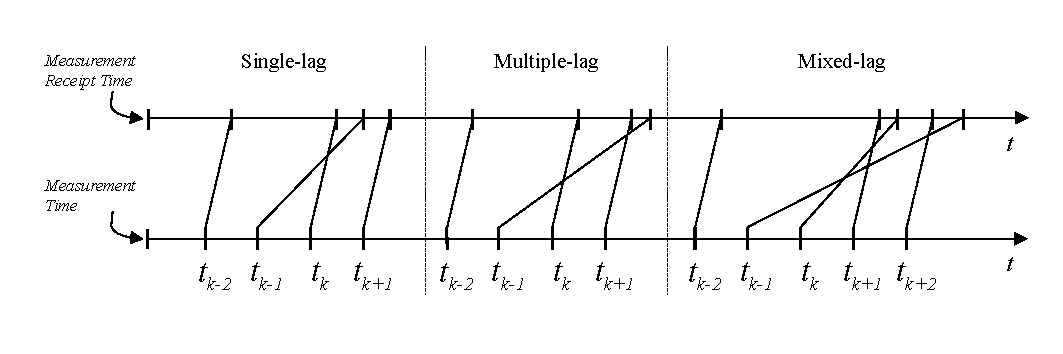
\includegraphics[scale=0.85]{Imagens/oosm.pdf}
	\caption[esquemas]{Different classes of out-of-sequence measurements irregularities}
	\label{fig:oosm}
\end{figure} 

\citep{Anxi2005} describes four different filtering approaches to deal with OOSM: reprocessing, that stores filter results to rollback with the time-delayed measurement; data buffering, that holds a set of measurements, greater than maximum expected lag, to be sorted before filtering; discarding data, that neglects time-delayed measurements; and directly updating, that uses the delayed information to update current state estimate. \citep{Bar-Shalom2000} used the last approach to describe an optimal filter for the single-lag case.

A summary of causes and effects that time delay causes in an estimator are illustrated in Figure \ref{fig:diagrama_delay}.

\begin{figure}[!htb]
	\centering
	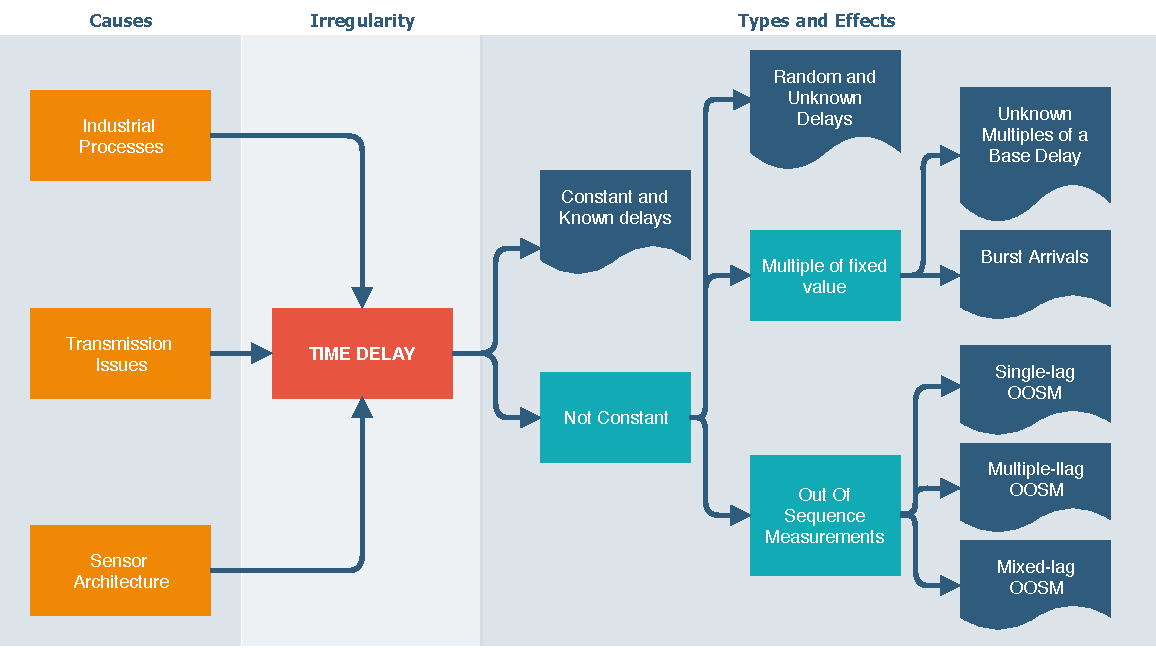
\includegraphics[scale=0.85]{Imagens/scheme_time-delay.pdf}
	\caption{Time delay diagram, showing the main causes (in orange) and effects (in dark blue) of time delay irregularity. The light blue boxes indicate different types that lead to different effects.}
	\label{fig:diagrama_delay}
\end{figure}

%\begin{figure}[!htb]
%	\begin{center}
%		
%		\begin{tikzpicture}[grow'=down,level distance=1.25in,sibling distance=.25in]
%		\tikzset{edge from parent/.style= 
%			{thick, draw, edge from parent fork down},
%			every leaf node/.style=
%			{draw,minimum width=1in,text width=1in,align=center,fill=orange!50},
%			every tree node/.style=
%			{draw,minimum width=1in,text width=1in,align=center,fill=blue!50}
%		}
%		
%		\Tree 
%		[.{Time Delay} 
%		{Transmission Issues} 
%		{Sensor Architecture} 
%		{Industrial Processes} 
%		]
%		
%		\end{tikzpicture}
%		
%	\end{center}
%	\caption{Irregular sampling diagram, showing the main causes (in orange) and effects (in blue) of irregularities}
%	\label{fig:diagrama_delay}
%\end{figure}	

\section{Packet Loss}

When data are being transmitted by a large network of sensors, there is a probability they can get lost in the way or they might arrive after a significant delay, which is equivalent to a loss for practical	 applications~\citep{Sinopoli2004}. Usually referred to as packet dropout/loss, missing or intermittent observations, they may happen due to node failures, network congestion, limited bandwidth or temporal failure. 
	
Mathematical description of packet dropouts can be carried out recursively, as described in~\citep{Sun2011}, by

\begin{align}
\centering
\begin{split}
z(t)=H(t)x(t)+v(t), \\
y(t) = \xi(t)z(t)+(1-\xi(t))y(t-1),
\end{split}
\end{align}

\noindent
where $z(t) \in \mathbf{R}^m$ is the measured output transmitted to the estimator, $v(t) \in \mathbf(R)^m$ is white noise, $y(t) \in \mathbf{R}^m$ is the measurement received by the estimator and $\xi(t) \sim Ber(p)$ is a Bernoulli random variable that takes the value 1 with probability $p$ and 0 with probability $1-p$. That is, when $\xi(t)$ is 1, there is no packet dropout. If $\xi(t)$ is 0, however, the latest output is used at current time, in a recursive fashion.

Another way of describing multiple packet dropouts is by limiting the amount of consecutive dropouts ~\citep{ShuliSun2008}, where the received measurements are defined by

\begin{equation}
\begin{split}
y(t) = 	& \xi(t)z(t) + (1-\xi(t))\xi(t-1)z(t-1)+...\\
		& + (1-\xi(t))(1-\xi(t-1))...(1-\xi(t-N+1))z(t-N), N \geq 1,\\
\end{split}
\end{equation}

Such a model dictates that the measurement used by the estimator will be only the most recent available, and the amount of missing observations is limited to $N$. This conclusion can be drawn by the fact that

\begin{equation}
\xi(t)+(1-\xi(t))\xi(t-1) + ... + (1-\xi(t))(1-\xi(t-1))...(1-\xi(t-N+1)) = 1.
\end{equation}

A summary of causes and effects that time delay causes in an estimator are illustrated in Figure \ref{fig:packet_loss}.

\begin{figure}[!htb]
	\centering
	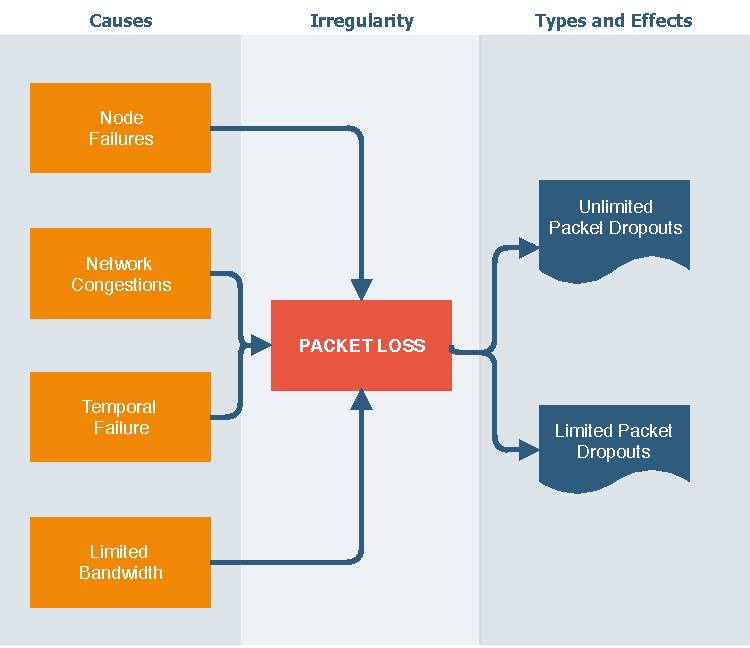
\includegraphics[scale=0.85]{Imagens/scheme_packet-loss.pdf}
	\caption{Packet loss diagram, showing the main causes (in orange) and effects (in dark blue) of time delay irregularity.}
	\label{fig:packet_loss}
\end{figure}


\section{Uncertain Observation}

For some applications, there is a chance that the observation signal sent to the estimator contains only noise. According to \citep{Jaffer1971}, it happens as a consequence of two situations: the observation was taken, but was lost during transmission, due to communication failures; or it was not transmitted at all, as it may happen for target tracking systems, for example, when the object being observed is not tracked at a sample time. An observation model for a sampled-data system can be described as

\begin{equation}
y(k) = \gamma(k)Cx(k) + Dv(k)
\end{equation}

\noindent
where $\gamma(k) \sim Ber(p(k))$ is a Bernoulli random variables, taking values of 0 or 1, with probabilities $p(k)$ and $1 - p(k)$, respectively.

Unlike the packet dropout problem, when the missing data are associated with the total absence of signal, the issue of uncertain observation has to be dealt with differently. A common approach is to detect the existence of signal prior to the assimilation, using a likelihood ratio test.  \citep{Middleton1968} proposes a joint approach to systematically detect and extract information from observation signals. If the estimator and detector are developed separately, te probability of false alarms is not used in the estimator, making it suboptimal. \citep{Nahi1969} developed an optimal recursive estimator, that uses the information of the random variable $\gamma$ in the algorithm, assuming it is independent and identically distributed. \citep{Hadidi1979} generalized the work of Nahi, for the case when the uncertainty of the signals presence is described by a Markovian sequence of binary random variables.

A summary of causes and effects that time delay causes in an estimator are illustrated in Figure \ref{fig:uncertain}.

\begin{figure}[!htb]
	\centering
	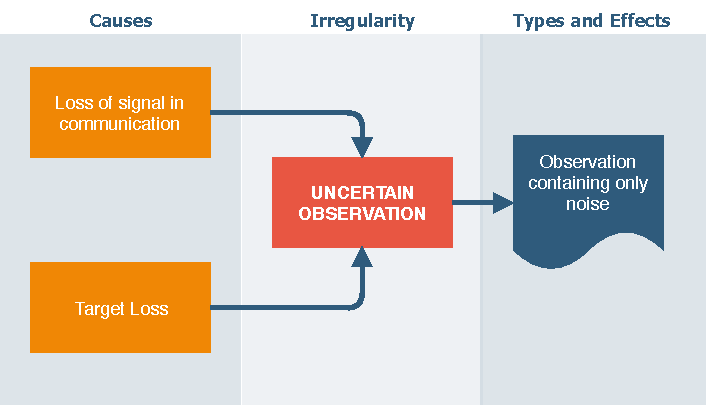
\includegraphics[scale=0.85]{Imagens/scheme_uncertain.pdf}
	\caption{Uncertain observations diagram, showing the main causes (in orange) and effects (in dark blue) of time delay irregularity.}
	\label{fig:uncertain}
\end{figure}

\section{Aperiodic Sampling}\label{sec:aperiodic}
	
All irregularities discussed so far may be present even in a periodic sampling scheme. However, for some applications, the sampling intervals are time-varying due to a variety of phenomena, causing what is called as aperiodic or asynchronous sampling. It can be the case of networked and embedded control systems, with unpredictable networked-induced issues, like irregular faults on samplers, oscillated loads, intermittent saturation or even variations in system components or parameters \citep{Shen2016}. Some imperfections may cause what is known as sampling jitter noise, which leads to time intervals being almost uniform. Automotive applications, radar imaging or event controlled systems are a few examples. In them, jitter noise happens due to sampling frequency similar to clock frequency, sampling requests delayed by the network or imperfect synchronization \citep{Eng2005}. For networks with a large amount of unsynchronized sensors, measurement arrival time intervals are randomly spaced and can be modeled as a stochastic process \citep{Micheli2002}. 

Sometimes, the system being observed has particularities that causes the aperiodic sampling. One example is seismology, where the spatial coordinates are irregularly sampled, because of natural obstacles \citep{Marvasti2001}. Other large scale systems, such as power grids, have sensors with a huge geographical separations, and different communication links to the estimation hub, which causes multiple and random inter-observation intervals \citep{Yan2017}.

Whereas for most cases, the non-uniformities in sampling time intervals appear as unwanted effects, there are cases when the sampling rule is designed to work irregularly. If there are limitations of communication resources (limited bandwidth or computation capacity) or a need for a reduced energy consumption, for example, time-driven sampling might be neglected in favor of an event-based scheme. In such strategy, an event-triggering mechanism is responsible for determining the sampling instants, according to Figure~\ref{fig:event-based}. For time-driven schemes, a clock triggers the transmission instants (a), while event-driven sampling instants depends on the sensor output itself with an optional feedback loop from the estimator, to assess estimation performance. Therefore, the trigger mechanism design provides a trade-off between performance and resource consumption efficiency, attracting a lot of research interest \citep{Liu2014}. The most common strategy for event-driven state estimation is the send-on-delta (SOD) \citep{Miskowicz2006}, which triggers the transmission when the value of the measured state deviates from the previous assimilated observation by an interval $\pm \Delta$, with $\Delta>0$. Other strategies were studied in \citep{Zou2017}. To avoid the risk of unexpected high amount of triggered measurements in a short period of time, which can lead to the dreaded Zeno behavior \citep{Tabuada2007}, lower-bounds can be defined both for the $\Delta$ value or for some explicit minimum inter-event time. 

\begin{figure}[!htb]
	\centering
	\begin{subfigure}
		\centering
		\text{(a)}\\
		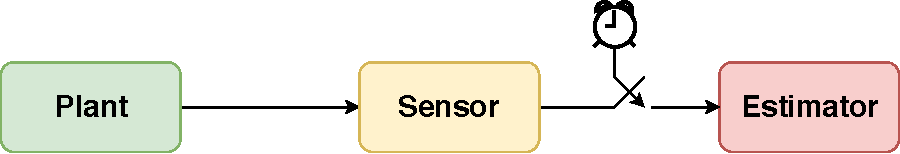
\includegraphics[width=0.75\textwidth]{Imagens/Event-based_clock.pdf}	
		\label{fig:evtb1}
	\end{subfigure}
	\vspace{1cm}\\
	\begin{subfigure}
		\centering
		\text{(b)}\\
		\vspace{0.25cm}
		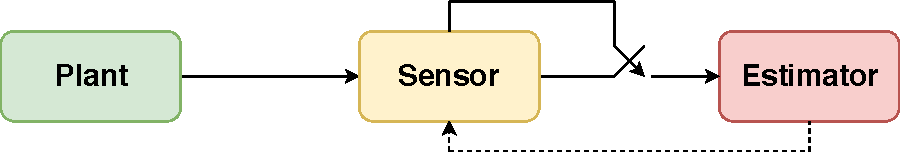
\includegraphics[width=0.75\textwidth]{Imagens/Event-based.pdf}
		%		\caption{}
		\label{fig:evtb2}
	\end{subfigure}
	\caption[Entradas]{Time-driven (a) and event-driven (b) sampling schemes. The connection between sensor and estimator is triggered by different mechanisms.}
	\label{fig:event-based}
\end{figure}

The measurement model of a linear system with aperiodic sampling can be defined as

\begin{equation}\label{eq:aperiodic}
y(t_k) = H(t_k)x(t_k) + v(t_k)
\end{equation}

\noindent
where $t_k$ is the random sampling time instant and the observation model matrix $H(t_k)$ is time-varying, if derived from the discretization of a continuous time system.

Generalizations of aperiodic sampling can be divided in two categories, based on how the estimator perceives the irregularity: as time noise added to a periodic pattern; or as a stochastic process, according to Figure~\ref{fig:aper-samp}. 

\begin{figure}[!htb]
	\centering
	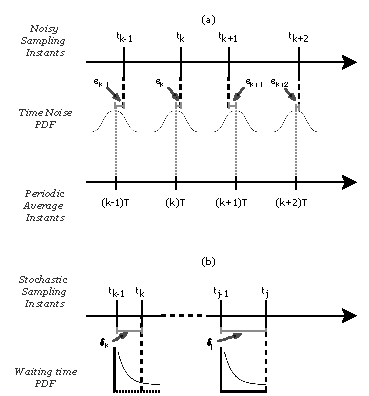
\includegraphics[width=0.85\textwidth]{Imagens/noisy_stoch_samp.pdf}	
	\caption[Entradas]{Aperiodic sampling categories: (a) noisy sampling over periodic intervals, with a Gaussian random variable added to expected time instants $kT$; and (b) sampling instants modeled as a stochastic process, with time intervals characterized by an exponential random variable (cumulative distribution functions are shown, for different $\lambda$ parameter values.)}
	\label{fig:aper-samp}
\end{figure}

For the first case, random time instants $t_k$ and the random time intervals $\delta_k$ can be defined as:

\begin{equation}
\begin{split}
t_k & \triangleq kT + \epsilon_k, \\
\delta_k & \triangleq t_k - t_{k-1} 
\end{split}
\end{equation}

\noindent
where $t_k$ is the k\textsuperscript{th} sampling instant, $T$ is the periodic time interval and $\epsilon_k$ is the deviation from the expected value $kT$. Note that, if the sampling time instants are a sequence of i.i.d Gaussian random variables, with variance $\sigma^2$, that is $t_k \sim \mathcal{N} (kT, \sigma^2)$, $\forall k \sim \mathbb{N}$, then the time interval random variable is Gaussian, with expected value $T$ and variance $2\sigma^2$, that is $\delta_k \sim \mathcal{N}(T,2\sigma^2)$.

For the stochastic process generalization, sampling time instants $t_k$ can be defined by the random time intervals $\delta_k$, such as:

\begin{equation}
\begin{split}
\delta_k & \triangleq t_k - t_{k-1}, \\
\delta_0 & \triangleq t_1
\end{split}
\end{equation}

\noindent
where random time intervals $\delta_k$ can be modeled, in the most flexible way, as a gamma probability density function, that is $\delta_k \sim \Gamma(k,\theta)$. If the shape parameter $k$ is a positive integer, it becomes an Erlang distribution, as used in \citep{Kanchanaharuthai2002}. For the most common case, where $k$ is held constant, the random time interval $\delta_k$ follows an exponential pdf the time sequence $t_k$ is represented by a Poisson stochastic process \citep{Micheli2002}.

A summary of causes and effects that time delay causes in an estimator are illustrated in Figure \ref{fig:aperiodic}.

\begin{figure}[!htb]
	\centering
	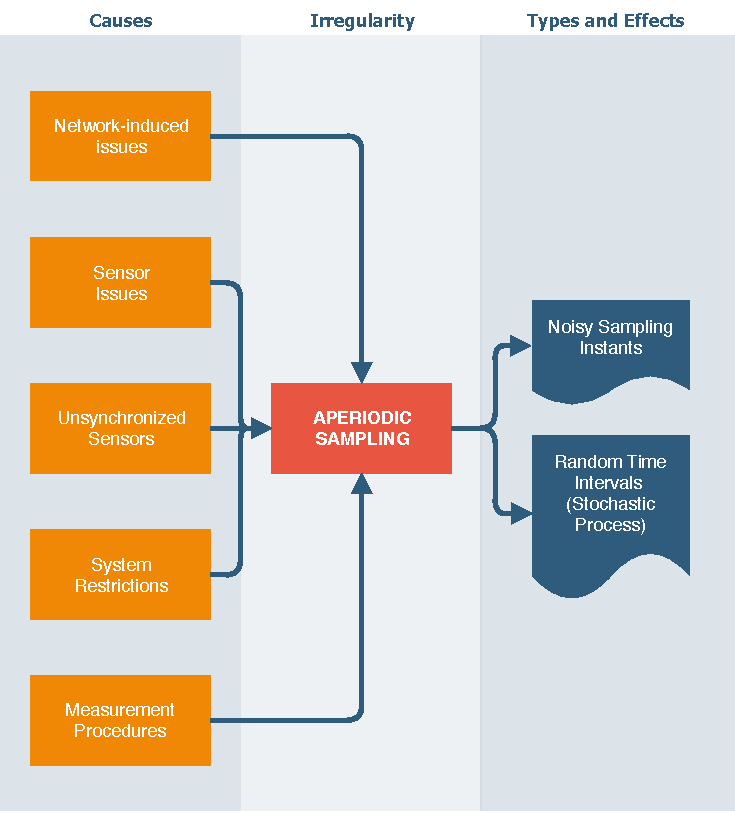
\includegraphics[scale=0.85]{Imagens/scheme_aperiodic.pdf}
	\caption{Uncertain observations diagram, showing the main causes (in orange) and effects (in dark blue) of time delay irregularity.}
	\label{fig:aperiodic}
\end{figure}

\section{Multi-Rate Sampling}

The last irregularity discussed is the multi-rate sampling. Generally, it refers to multiple sensors measuring the same system at different sampling rates. Many industrial processes need to control challenging variables that can be measured by online instruments that provide regular, fast rate and delay free information, but with low precision. Therefore, more accurate data are needed and usually available after slow and irregular laboratory analysis \citep{Penarrocha2012, Fatehi2017}. The combination of both sources of measurements leads to a multi-rate sampling scenario. 

A more common approach is the use of various sensors measuring the same physical information, to obtain better estimates, which has been drawing attention from real world applications, such as target tracking, robotics, surveillance and military. For such strategy, the sampling rates perceived by the estimator are often different from one another. The work of \citep{Lin2016} and the references therein provide a wide coverage of scenarios derived from multi-sensor multi-rate systems. 

Figure \ref{fig:multi-rate} illustrates the ways multi-rate sampling can manifest in a system. The different rates from the various sensor devices can be periodic (a), aperiodic (b) or even a mixture of both, as is the case for most industrial applications with laboratory analysis.

\begin{figure}[!htb]
	\centering
	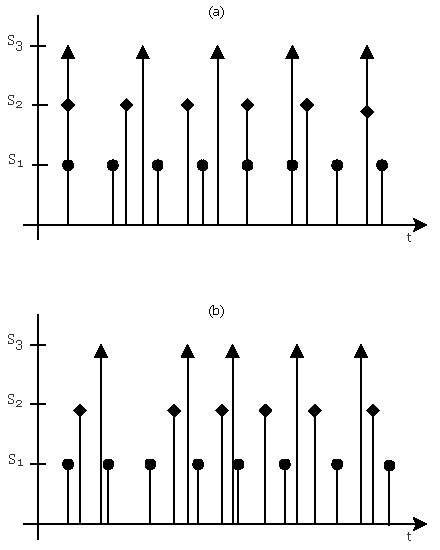
\includegraphics[width=0.5\textwidth]{Imagens/multi_rate.pdf}	
	\caption[Entradas]{(a) Periodic multi-rate and (b) aperiodic sampling scheme.}
	\label{fig:multi-rate}
\end{figure}

Aperiodic sampling rates can be described the same way as in Section \ref{sec:aperiodic}, by equation \ref{eq:aperiodic}. Periodic multi-rate measurements can be modeled as

\begin{equation}
	y_i(k_i) = H_i(x(k_i)) + v_i(k_1)
\end{equation}

\noindent
where $y_i(k_i)$ represents the $k_i^{th}$ observation from sensor $i$ and $H_i$ is the discrete measurement model matrix.

A summary of causes and effects that time delay causes in an estimator are illustrated in Figure \ref{fig:multi_rate}.

\begin{figure}[!htb]
	\centering
	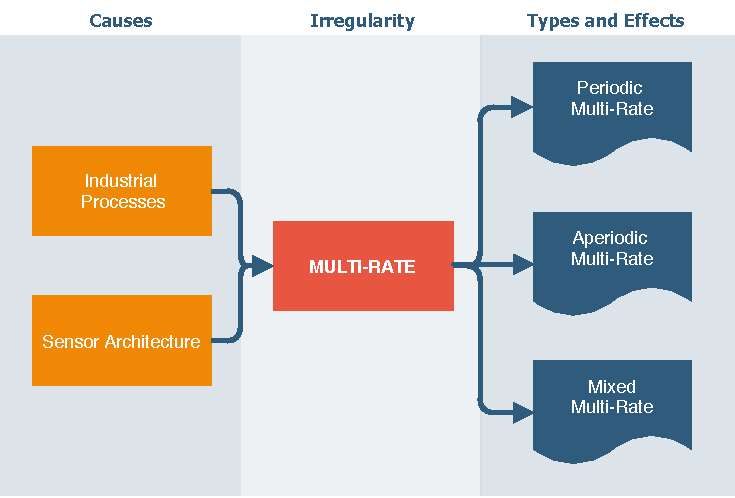
\includegraphics[scale=0.85]{Imagens/scheme_multi-rate.pdf}
	\caption{Uncertain observations diagram, showing the main causes (in orange) and effects (in dark blue) of time delay irregularity.}
	\label{fig:multi_rate}
\end{figure}


\clearpage
%%%

%%% Capítulo 3
%!!!!!!!!!!!!!!!!!!!!!!!!!!!!!!!!!!!!!!!     ATENÇÃO     !!!!!!!!!!!!!!!!!!!!!!!!!!!!!!!!!!!!!!!!!!!
%	Para saber o número da primeira página do capítulo 3, verifique o número da última página
% colocado no capítulo 2. Lembrando que cada capítulo se inicia em ímpar.
%!!!!!!!!!!!!!!!!!!!!!!!!!!!!!!!!!!!!!!!!!!!!!!!!!!!!!!!!!!!!!!!!!!!!!!!!!!!!!!!!!!!!!!!!!!!!!!!!!!!
%%% Força a contagem da página.
\clearpage
\setcounter{page}{5}
%%%
%------------------------------------------------------------------------------
\hypertarget{lcap3}{}
\chapter{Irregular Sampling}
\vspace{-1cm} \label{cap3}

%\begin{flushright}
%\begin{minipage}{0.7\linewidth}
%\emph{``Quando uma criatura humana desperta para um grande sonho e
%sobre ele lan�a toda a for�a de sua alma, todo o universo conspira a
%seu favor.''}
%\end{minipage}
%\end{flushright}
%
%\begin{flushright}
%{Goethe}
%\end{flushright}

%\vspace{1cm}

%%Colocar uma descri��o do cap�tulo aqui!
%\section{Introdu��o}\label{sec int_cap_2}

In the last chapter, we reviewed the main motivations and advantages behind the sensor fusion field of science, as well as its techniques. Despite all the growth and benefits obtained by fusing data from multiple sensors, some challenges naturally appear. For the state estimation problem for sampled-data systems, a common challenge is related to sampling irregularities introduced in a network.

In this chapter, we review the irregular sampling problem. First, the concept of irregular sampling adopted in this study is discussed. In Section \ref{sec:intro} we categorize the different types of irregularities that may occur in sampling and discuss their main causes and characteristics. Then, in Secton~\ref{sec:irreg_types}, each irregularity is further discussed, with examples, mathematical models and their subdivisions, where applicable. We end this chapter with a discussion of time synchronization in Section~\ref{sec:sync}, which is needed to guarantee a common time scale for all nodes in a network, enabling the irregularities to be dealt with appropriately.

\section{Definition of Irregular Sampling}

Most of the systems studied in estimation and control theories take place in an analog environment with dynamics evolving according to continous-time differential equations. However, due to the many benefits of digital technology implementations, their signal must be sampled in order to be processed, giving rise to the so-called \textit{sampled-data systems}. 

In practice, the sampling process is modeled by a sampler and a data hold device, that enables signal reconstruction. The most common data hold configuration is the zero-order holder (ZOH), that outputs a constant value equals to the signal value at the sampling instant during the whole time interval, until the next sample is available. 
%Therefore, the output of a sampler that transmits data every $T$ seconds and a ZOH is given by~\citep{Phillips1995}
%
%\begin{equation}\label{eq:sampled}
%\bar{f}(t)=f(0)[u(t)-u(t-T)]+f(T)[u(t)-u(t-2T	)]+f(2T)[u(t-2T)-u(t-3T)]+ \ ...,
%\end{equation}
%
%\noindent
%where $\bar{f}(t)$ represents the reconstructed sampled signal, $f(t)$ is the original continuous-time signal and $u(t)$ is the unit-step function. Taking the Laplace transform of (\ref{eq:sampled}) we have
%
%\begin{align}\label{eq:sampled_laplace}
%\bar{F}(s)=\mathcal{L}[f(t)]&=f(0)\left[\frac{1}{s}-\frac{e^{-Ts}}{s}\right]+f(T)\left[\frac{e^{-Ts}}{s}-\frac{e^{-2Ts}}{s}\right] + f(2T)\left[\frac{e^{-2Ts}}{s}-\frac{e^{-3		Ts}}{s}\right] + \ ... \notag \\
%&= \left[\sum_{n=0}^\infty f(nT) e^{-nTs}\right] \left[\frac{1-e^{-Ts}}{s}\right].
%\end{align}
%
%Only the first term of (\ref{eq:sampled_laplace}) is dependent on $f(t)$ and thus can be interpreted as the sampler, whereas the second term represents the ZOH. Note that neither exists alone, since the real physical signal is composed by both terms. Taking the inverse Laplace transform of the sampler term yields
%
%\begin{equation}\label{eq:sampled_invlaplace}
%\mathcal{L}^{-1}\left[\sum_{n=0}^\infty f(nT) e^{-nTs}\right] = f(0)\delta(t)+f(T)\delta(t-T)+f(2T)\delta(t-2T)+ \ ... \ ,
%\end{equation}
%
%\noindent
%where $\delta(t)$ is the unit impulse function, also known as Dirac delta function. Although it does not represent a real signal, (\ref{eq:sampled_invlaplace}) is referred to as the \textit{ideal sampler}~\citep{Phillips1995}.

Thus the state observations of a sampled-data system can be modeled as

\begin{equation}\label{eq:reg_sampled_obs}
y(t) = g(x(kT),v(kT),kT), \quad \textrm{for } kT\leq t<(k+1)T,
\end{equation}

\noindent
where $g\!\!: \mathbb{R}^n \times \mathbb{R}^r \times \mathbb{R^+} \rightarrow \mathbb{R}^m $ represents the observation model, $x(kT) \in \mathbb{R}^n$ is the state vector, $v(kT) \in \mathbb{R}^m$ is the measurement error, $k \in \mathbb{N}$ is the discrete-time index and $T \in \mathbb{R^+}$ is the sampling interval. 

Therefore, a sampled-data system is regularly sampled if its observation model can be modeled by (\ref{eq:reg_sampled_obs}), as a consequence of an \textit{ideal sampler}. In other words, in this study we refer to \textit{regular sampling} as measurements being taken periodically, with single-rate and transmitted without time-delay and any loss of information. Anything else will be framed as \textit{irregular sampling}.

\section{Contextualization}\label{sec:intro}

Sampling irregularities may occur due to a variety of issues. Sometimes they occur as undesired side effects of using large sensor networks architectures and others due to deliberate non-uniform sampling schemes. In this section we try to categorize and review the main irregularities observed in practice. The diagram in Figure \ref{fig:diagrama2} provides a simplified overview of them, separated by their sources.

\begin{figure}[!htb]
\centering
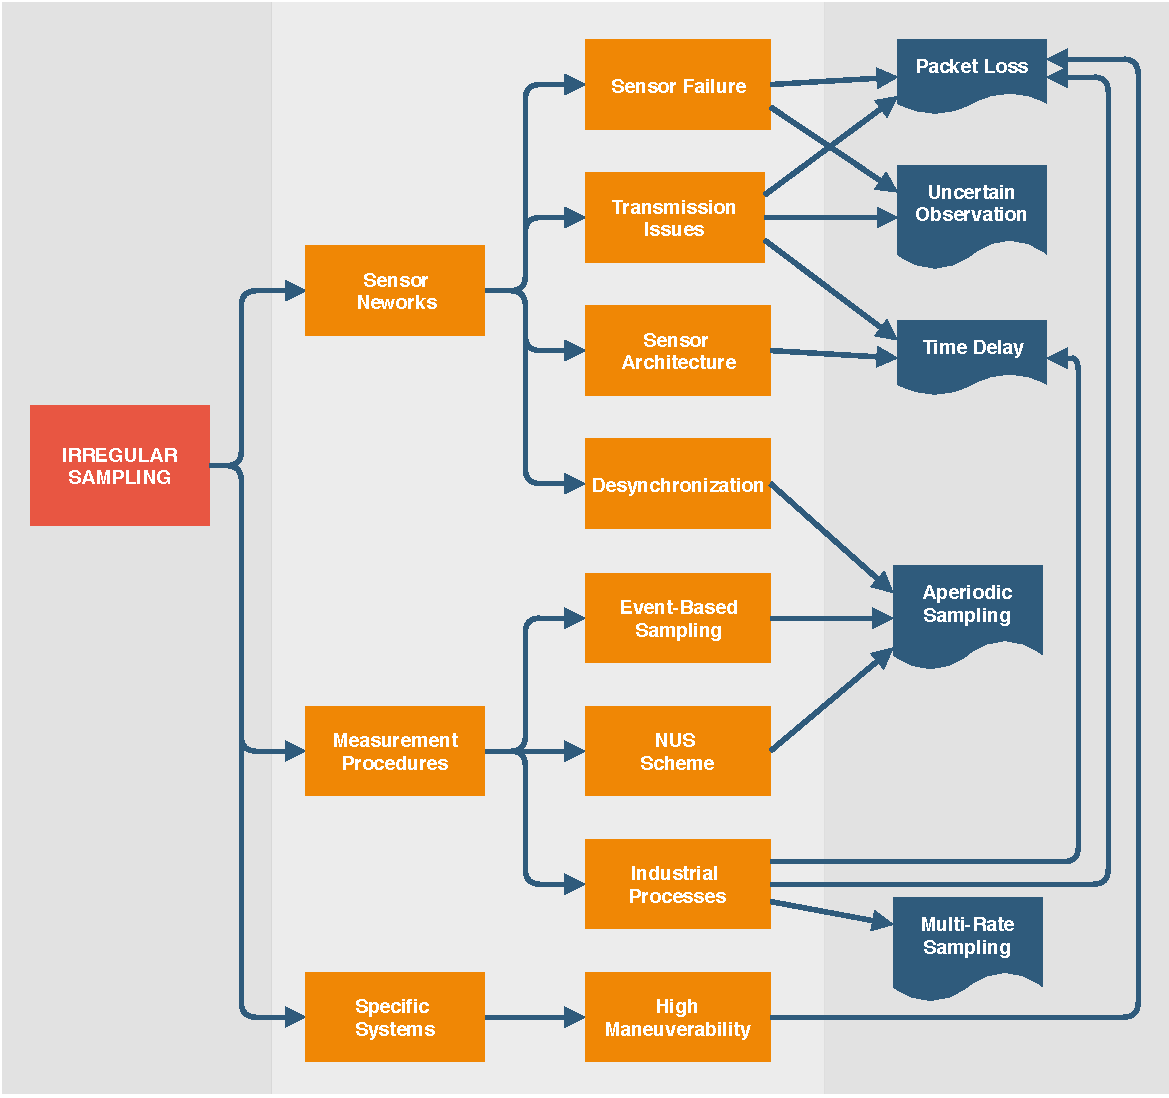
\includegraphics[width=\textwidth]{Imagens/irreg_sampling.pdf}
\caption[Irregular sampling diagram]{Irregular sampling diagram, showing the main causes (in orange) and effects (in blue)}
\label{fig:diagrama2}
\end{figure}

The use of imperfect communication networks seems to be the main cause of irregular sampling. Unreliable communication channels may lead to random time delays and loss of information, specially if data are transmitted using a common medium \citep{Sahebsara2007, Moayedi2011}. In case they get randomly interrupted during transmission or if a sensor fails at some point, the signal received may predominantly contain noise, causing uncertain observation or packet dropouts \citep{Hadidi1979, Wang2009}. Systems that are observed by a large number of desynchronized sensors will provide observations at random time intervals \citep{Micheli2002}. If they are synchronized but designed to operate in a centralized fashion, there is a chance that different time delays are produced due to distinct transmission routes for each sensor \citep{Bar-Shalom2000, Challa2003, Anxi2005}. 

However, the communication networks shall not always be held responsible. Some applications are designed to be measured in an irregular way. In event-based schemes, for example, the measurements are transmitted only when certain conditions are met \citep{Liu2014,Zou2017}. Such approach can reduce communication resource consumption substantially \citep{Hu2017}, but it will cause aperiodic sampling. Non-Uniform Sampling (NUS) is also intentionally used as an alias detection method \citep{Kunoh2015} or to enhance the spectral resolution of signals, largely used in Nuclear Magnetic Resonance (NMR) spectroscopy analysis \citep{Hyberts2013}, for instance. In other situations, due to the nature of the process being observed, the measurement strategy relies on different procedures. For a lot of chemical processes, for instance, the variables can be measured in an online, fast rate and delay free fashion, but providing inaccurate data. Therefore, laboratory analyses are used to improve estimation quality, but  usually at slower rates, sometimes irregularly and with possible time delays \citep{Fatehi2017}. Other industrial applications suffer from the same dilemma, and the sampling scheme ends up with a multi-rate data transmission, with random time delays and possibly measurement scarcity \citep{Penarrocha2012}. 


Finally, sampling irregularities might also appear due to a specific nature of a system. In some high maneuverable target-tracking applications, for example, there is a chance that the sensor misses the target, transmitting only noise, leading to the so called uncertain observation issue \citep{Wang2009, Chen2013}.

Whatever the reason for the irregularities, data need to be properly associated to the same observed phenomenon in order to be fused into knowledge. A crucial part of this association is the temporal synchronization of information on the time when the observations were taken \citep{Ping2003}. Most sensor fusion methods for irregularly sampled systems rely on the correct timestamps to develop modifications in classical algorithms. If observations are imprecisely time stamped, some alternatives have been proposed to incorporate some aspects of that imprecision in the estimation method \citep{Julier2005, Huck2011}. Still, some knowledge about the irregularity is assumed to be known. Alternatively, many techniques for time synchronization can be performed, to ensure a common temporal reference for all the sensors. 

On the next sections, we review the main irregular sampling types and the main approaches to deal with time synchronization in sensor networks.

\section{Types of Sampling Irregularity}\label{sec:irreg_types}

\subsection{Time Delay}

Signal time delays might affect state estimation in various ways and due to different reasons, as shown in Figure \ref{fig:diagrama_delay}. In some cases, delays can be modeled as constant and known \citep{Lu2005}. Alternatively they might not be known and constant, but still multiple of a fixed value. In such cases, observations might be received in a burst, when more than one packet arrive between two consecutive sampling instants. State estimation algorithms can be adapted to handle such irregularity by using only the latest measurement and discarding all others, or implementing a buffer to iterate over all received packets \citep{Moayedi2011}.

\begin{figure}[!htb]
	\centering
	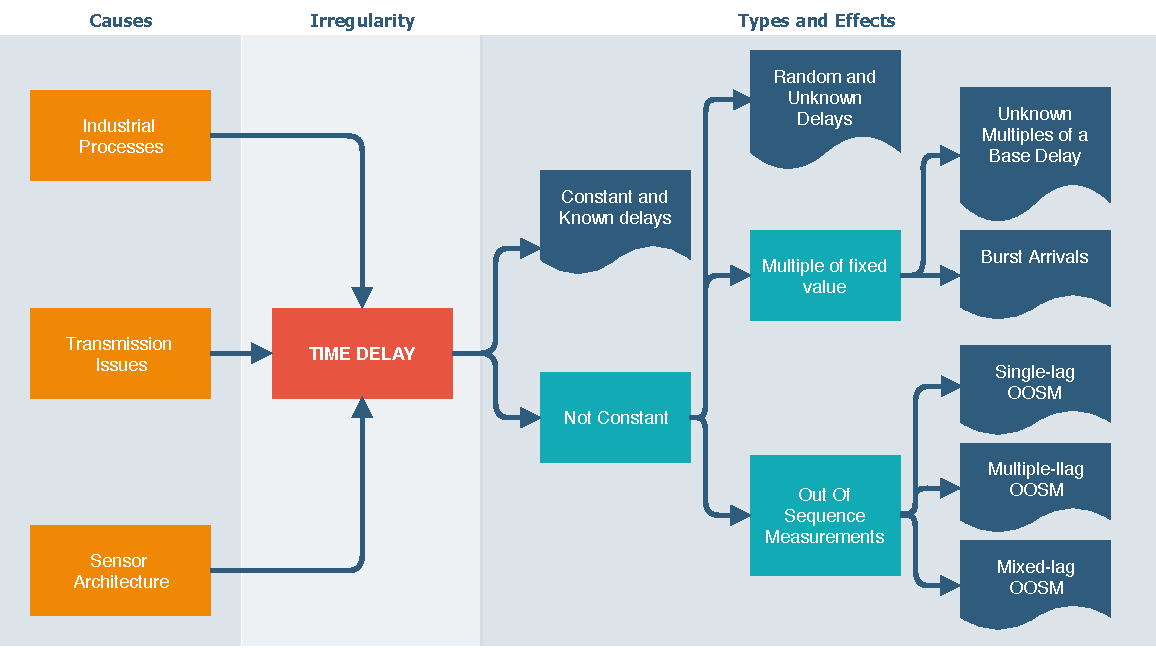
\includegraphics[width=\textwidth]{Imagens/scheme_time-delay.pdf}
	\caption[Time delay diagram]{Time delay diagram, showing the main causes (in orange) and effects (in dark blue) of time delay irregularity. The light blue boxes indicate different types that lead to different effects.}
	\label{fig:diagrama_delay}
\end{figure}

%Time-delay systems (TDS) are probably the most common mathematical representation to time delays in practice. The works of \citep{Richard2003, Fridman2014} and the references therein provide a good coverage of the subject. In TDSs, there might be delays in the input or in the output signals, introduced by communication networks, or even in the states themselves. The latter phenomenon is called system with aftereffect or dead-time. Since we are studying the irregular sampling issue, only signal delays are relevant to us. A summary of causes and effects that time delay causes in an estimator are illustrated in Figure \ref{fig:diagrama_delay}.

%Considering delays in the measurement model only, \citep{Lu2005} studied the estimation problem when they are constant and known. They describe a discrete linear measurement model observed by $l$ different systems with delays as 
%
%\begin{equation}\label{eq:delay_model}
%	y_i(kT)=H_i(kT)x(t_i)+v_i(kT)
%\end{equation}
%
%
%\noindent
%where $k$ is the discrete-time index of measurements, $T$ is the sampling interval, $i=0,\ 1,\ ...,\ l$ and $l$ is the number of different known delays for each observation system. $y_i(kT) \in \mathbb{R}^{p_i}$ are delayed measurements and $v_i(kT) \in \mathbb{R}^{p_i}$, the measurement noise. The known delayed time instants are given by $t_i=t_{i-1}-d_i$, with $d_0=0$, $d_i>0$ for $i>0$ and $t_0=kT$. For a given time instant $kT$, $y_i(kT)$ represents the observation of state $x(t_i)$ at time $kT$, with total delay $\sum_{k=1}^{i}d_k$. Thus, if $T \geq d_1 \ + \ ...\  + \ d_l$, the complee observation vector of state $x(t_i)$ at time $kT$, becomes $[y_0^T(kT) \ ... \ y_l^T(kT)]^T$. On the other hand, if the sampling interval is smaller than the delay of one or more observation system, that is $ d_1 \ + \ ... \ + \ d_{i-1}\leq T < d_1 \  + ... \ + \ d_l$, then observation of the system is given by $[y_0^T(kT) \ ... \ y_{i-1}^T(kT) \ 0 \ ... \ 0]^T$.
%



However, in many applications the measurements are received by the estimator with irregular and unknown delays, although taken at regular time intervals. In such cases, time delays can be interpreted as a stochastic process $d(k)$, varying randomly throughout time \citep{Han2009}.

% describes a discrete-time measurement model for random delayed observations as
%
%\begin{equation}\label{eq:delay_model2}
%y(k) = H(k)x(k-d(k))+L(k)v(k)
%\end{equation}
%
%\noindent
%where $d(k) \in \mathbb{N}$ is a random but bounded time delay, assumed to be a discrete-time Markov Chain with finite space $\{0,\ d\}$, observable at each sampling time $k$.

Multiples of a known lag or not, delayed measurements from a multisensor system can arrive disordely, which leads to the sampling irregularity commonly known as out-of-sequence-measurements (OOSM). It can be classified in three ways, depending on the number of lags, according to Figure~\ref{fig:oosm}. 

\begin{figure}[!htb]
	\centering
	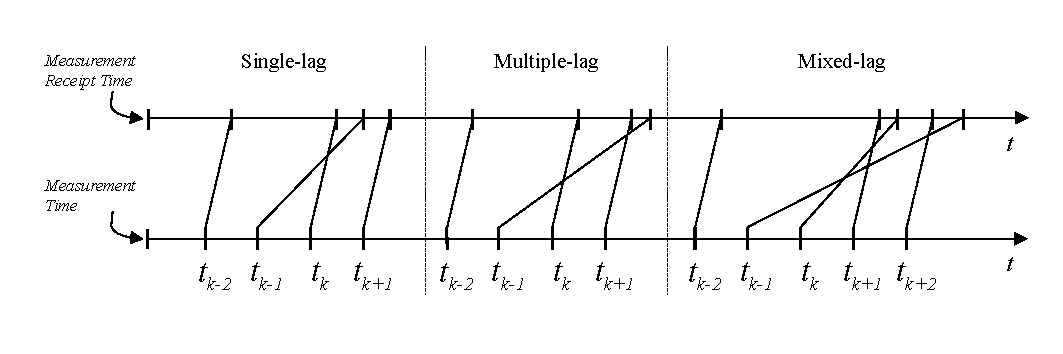
\includegraphics[width=0.95\textwidth]{Imagens/oosm.pdf}
	\caption{Different classes of out-of-sequence measurements irregularities}
	\label{fig:oosm}
\end{figure} 

\citep{Anxi2005} describes four different filtering approaches to deal with OOSM: reprocessing, that stores filter results to rollback with the time-delayed measurement; data buffering, that holds a set of measurements, greater than the maximum expected lag, to be sorted before filtering; discarding data, that neglects time-delayed measurements; and directly updating, that uses the delayed information to update current state estimate. \citep{Bar-Shalom2000} used the last approach to describe an optimal filter for the single-lag case.


\subsection{Packet Loss}

When data are being transmitted by a large network of sensors, there is a probability that they get lost in the way or they might arrive after a significant delay, which is equivalent to a loss for practical	 applications~\citep{Sinopoli2004}. Usually referred to as packet dropout or loss, missing or intermittent observations or scarse measurements~\citep{Albertos2004}, they may happen due to node failures, network congestion, limited bandwidth or temporal failure. A summary of causes and effects associated with packet loss are shown in Figure \ref{fig:packet_loss}.

\begin{figure}[!htb]
	\centering
	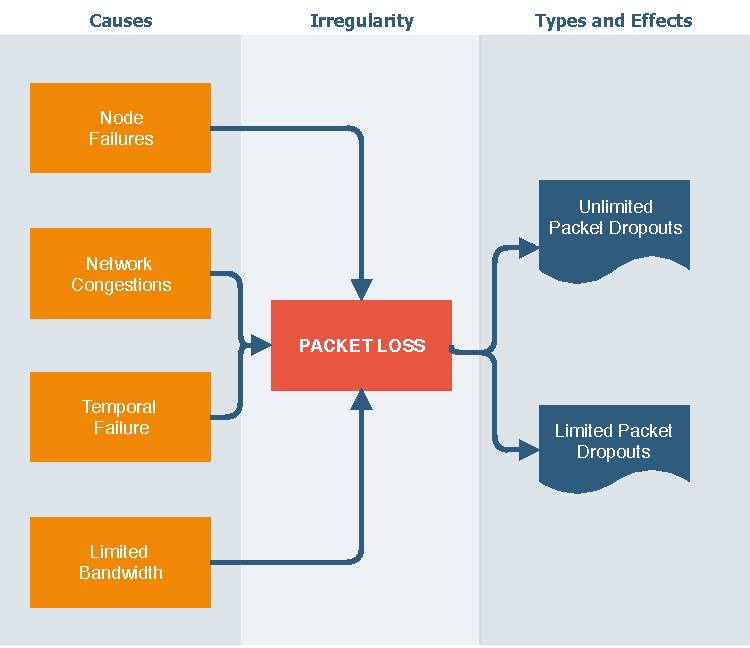
\includegraphics[width=0.75\textwidth]{Imagens/scheme_packet-loss.pdf}
	\caption[Packet loss diagram]{Packet loss diagram, showing the main causes (in orange) and effects (in dark blue) of time delay irregularity.}
	\label{fig:packet_loss}
\end{figure}

	
Mathematical description of packet dropouts can be carried out recursively, as described in~\citep{Sun2011}, by

\vspace{-2pt}
\begin{equation}
\centering
y(k)  = \xi(k)z(k)+(1-\xi(k))y(k-1),
\end{equation}

\noindent
where $z(k) \in \mathbb{R}^m$ is the $k$-th measured output transmitted to the estimator, $y(k) \in \mathbb{R}^m$ is the $k$-th measurement received by the estimator and $\xi(k) \sim Ber(p)$ is a Bernoulli stochastic process that takes the value 1 with probability $p$ and 0 with probability $1-p$. That is, when $\xi(k)$ is 1, there is no packet dropout. If $\xi(k)$ is 0, however, the latest output is used at current time, in a recursive fashion.

Another way of describing multiple packet dropouts is by limiting the amount of consecutive dropouts ~\citep{ShuliSun2008}, where the received measurements are defined by
\vspace{-1pt}
\begin{equation}
\begin{split}
y(k) = 	& \xi(k)z(k) + (1-\xi(k))\xi(k-1)z(k-1) + (1-\xi(k))(1-\xi(k-1))\xi(k-2)z(k-2)  +\ ...\\
		& + (1-\xi(k))(1-\xi(k-1))...(1-\xi(k-N+1))\xi(k-N)z(k-N), \quad N \geq 1.\\
\end{split}
\end{equation}

Such a model dictates that the measurement used by the estimator will be only the most recent available, and the amount of missing observations is limited to $N$. 

\subsection{Uncertain Observation}\label{sec:uncertain}

For some applications, there is a chance that the observation signal sent to the estimator contains only noise. According to \citep{Jaffer1971}, it happens as a consequence of two situations: the observation was taken, but it was lost during transmission, due to communication failures; or it was not transmitted at all, as it may happen for target tracking systems, for example, when the object being observed is not tracked at a sample time. A summary of causes and effects associated with uncertain observations are shown in Figure \ref{fig:uncertain}.

\begin{figure}[!htb]
	\centering
	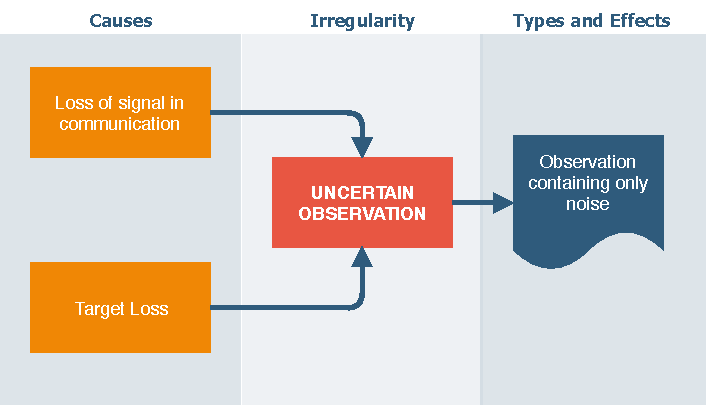
\includegraphics[width=0.75\textwidth]{Imagens/scheme_uncertain.pdf}
	\caption[Uncertain observations diagram]{Uncertain observations diagram, showing the main causes (in orange) and effects (in dark blue) of time delay irregularity.}
	\label{fig:uncertain}
\end{figure}

An observation model for a sampled-data system with uncertain observations can be described as

\begin{equation}
y(k) = \xi(k)z(k) + v(k)
\end{equation}

\noindent
where $z(k) \in \mathbb{R}^m$ is the $k$-th measured output transmitted to the estimator, $y(k) \in \mathbb{R}^m$ is the $k$-th measurement received by the estimator and $\xi(k) \sim Ber(p(k))$ is a Bernoulli random variables, taking values of 0 or 1, with probabilities $p(k)$ and $1 - p(k)$, respectively.

Unlike the packet dropout problem, when the missing data are associated with the total absence of signal, the issue of uncertain observation has to be dealt with differently. A common approach is to detect the existence of signal prior to the assimilation, using a likelihood ratio test.  \citep{Middleton1968} proposes a joint approach to systematically detect and extract information from observation signals. If the estimator and detector are developed separately, the probability of false alarms is not used in the estimator, making it sub-optimal. \citep{Nahi1969} developed an optimal recursive estimator that uses the information of the stochastic process $\xi(k)$ in the algorithm, assuming its sequence is independent and identically distributed. \citep{Hadidi1979} generalized the work of Nahi, for the case when the uncertainty of the signals presence is described by a Markovian sequence of binary random variables.



\subsection{Aperiodic Sampling}\label{sec:aperiodic}
	
All irregularities discussed so far may be present even in a periodic sampling scheme. However, for some applications, the sampling intervals are time-varying due to a variety of phenomena, causing the so-called aperiodic or asynchronous sampling. A summary of causes and types of aperodic sampling is presented Figure \ref{fig:aperiodic}.

\begin{figure}[!htb]
	\centering
	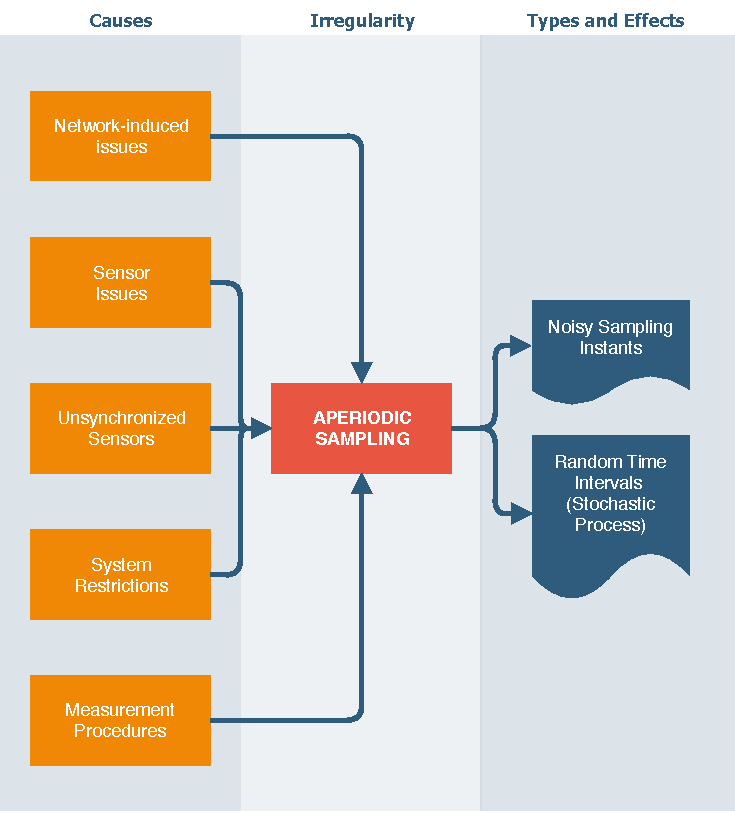
\includegraphics[width=0.75\textwidth]{Imagens/scheme_aperiodic.pdf}
	\caption[Aperiodic sampling diagram]{Aperiodic sampling diagram, showing the main causes (in orange) and types (in dark blue) of irregularity.}
	\label{fig:aperiodic}
\end{figure}

Usually such irregularity happens in networked and embedded control systems, with unpredictable networked-induced issues, such as irregular faults on samplers, oscillated loads, intermittent saturation or even variations in system components or parameters \citep{Shen2016}. Some imperfections may cause what is known as sampling jitter noise, which leads to time intervals being almost uniform. Automotive applications, radar imaging or event controlled systems are a few examples. In such cases, jitter noise happens due to a sampling frequency similar to the clock frequency; to sampling requests delayed by the network; or to imperfect synchronization \citep{Eng2005}. For networks with a large amount of unsynchronized sensors, measurement arrival time instants are randomly spaced and can be modeled as stochastic processes \citep{Micheli2002}. Sometimes, the system being observed has particularities that causes the aperiodic sampling. One example is seismology, where the spatial coordinates are irregularly sampled, because of natural obstacles \citep{Marvasti2001}. Other large scale systems, such as power grids, have sensors with huge geographical separations and different communication links to the estimation hub, causing multiple and random inter-observation intervals \citep{Yan2017}.

Whereas for most cases the variations in sampling time intervals appear as unwanted effects, there are cases when the sampling rule is designed to work aperiodically. If there are limitations of communication resources (limited bandwidth or computation capacity, for instance) or a need for reduced energy consumption, time-driven sampling might be replaced in favor of an event-based scheme. In such strategy, an event-triggering mechanism is responsible for determining the sampling instants, as depicted in Figure~\ref{fig:event-based}. For time-driven schemes, a clock triggers the transmission instants, while event-driven sampling instants depends on the sensor output itself with an optional feedback loop from the estimator to assess estimation performance. Therefore, the trigger mechanism design provides a trade-off between performance and resource consumption efficiency, attracting a lot of research interest \citep{Liu2014}. The most common strategy for event-driven state estimation is the send-on-delta (SOD) \citep{Miskowicz2006}, which triggers the transmission when the value of the measured state deviates from the previous assimilated observation by an interval $\pm \Delta$, with $\Delta>0$. Other strategies were studied in \citep{Zou2017}. To avoid the risk of unexpected high amount of triggered measurements in a short period of time, lower-bounds can be defined both for the $\Delta$-value or for some explicit minimum inter-event time.



\begin{figure}[!htb]
	\centering
	\begin{subfigure}
		\centering
		\text{(a)}\\
		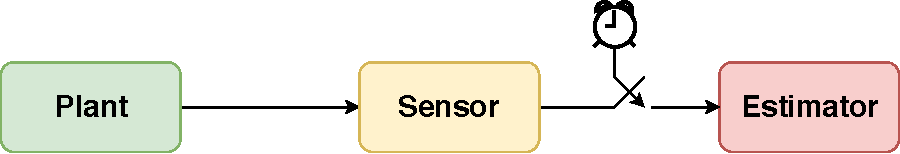
\includegraphics[width=0.75\textwidth]{Imagens/Event-based_clock.pdf}	
		\label{fig:evtb1}
	\end{subfigure}
	\vspace{1cm}\\
	\begin{subfigure}
		\centering
		\text{(b)}\\
		\vspace{0.25cm}
		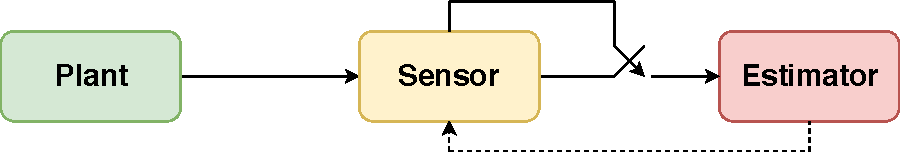
\includegraphics[width=0.75\textwidth]{Imagens/Event-based.pdf}
		%		\caption{}
		\label{fig:evtb2}
	\end{subfigure}
	\caption[Time-driven and event-driven sampling schemes]{(a) Time-driven and (b) event-driven sampling schemes. The connection between sensor and estimator is triggered by different mechanisms.}
	\label{fig:event-based}
\end{figure}




The measurement model with aperiodic sampling can be defined as

\begin{equation}\label{eq:aperiodic}
y(t_k) = z(t_k) + v(t_k)
\end{equation}

\noindent
where $t_k$ is the random sampling time instant and $z(t_K)$ is the transmitted measurement.

Generalizations of aperiodic sampling can be divided in two categories, based on how the estimator perceives the irregularity: as time signal noise added to a periodic pattern; or as a stochastic process, as illustrated in Figure~\ref{fig:aper-samp}. 

\begin{figure}[!htb]
	\centering
	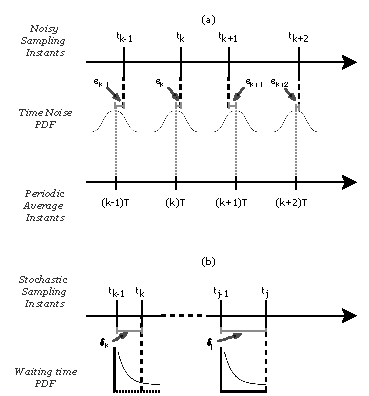
\includegraphics[width=0.8\textwidth]{Imagens/noisy_stoch_samp.pdf}	
	\caption[Two models of aperiodic sampling]{Two models of aperiodic sampling: (a) noisy sampling over periodic intervals, with a Gaussian random variable added to expected time instants $kT$; and (b) sampling instants modeled as a stochastic process, with time intervals characterized by an exponential random variable. For (b), the cumulative distribution functions are shown, for different $\lambda$ parameter values.}
	\label{fig:aper-samp}
\end{figure}

For the first case, random time instants $t_k$ and the random time intervals $\delta_k$ can be defined as:
\vspace{-1pt}
\begin{equation}
\begin{split}
t_k & \triangleq kT + \epsilon_k, \\
\delta_k & \triangleq t_k - t_{k-1} 
\end{split}
\end{equation}

\noindent
where $t_k$ is the $k$\textsuperscript{th} sampling instant, $T$ is the constant time interval and $\epsilon_k$ is the deviation from the expected value $kT$. Note that, if the sampling time instants are a sequence of i.i.d Gaussian random variables, with variance $\sigma^2$, that is $t_k \sim \mathcal{N} (kT, \sigma^2)$, $\forall k \sim \mathbb{N}$, then the time interval random variable is Gaussian, with expected value $T$ and variance $2\sigma^2$, that is $\delta_k \sim \mathcal{N}(T,2\sigma^2)$.

For the stochastic process generalization, sampling time instants $t_k$ can be defined by the random time intervals $\delta_k$, such as:

\begin{equation}
\begin{split}
\delta_k & \triangleq t_k - t_{k-1}, \\
\delta_0 & \triangleq t_0
\end{split}
\end{equation}

\noindent
where random time intervals $\delta_k$ can be modeled, in the most flexible way, as a gamma probability density function, that is $\delta_k \sim \Gamma(\kappa,\theta)$. If the shape parameter $\kappa$ is a positive integer, then it becomes an Erlang distribution, as done in \citep{Kanchanaharuthai2002}. For the most common case, where $\kappa$ is held constant, the random time interval $\delta_k$ follows an exponential PDF and the time sequence $t_k$ is represented by a Poisson stochastic process \citep{Micheli2002}. In fact, Micheli and Jordan proved that for a network with $N$ unsynchronized sensors with sampling period $T$, the waiting time between two arrivals tends, in distribution, to the exponential random variable, that is 
$\delta_k \sim \mathcal{E} (\lambda)$, where $\lambda = N/T$, as $N$ tends to infinity. In such cases, the expected value of the RV $\delta_k$ is $E[\delta_k] = 1/\lambda$ and its variance is $Var[\delta_k] = 1/\lambda^2$.


\subsection{Multi-Rate Sampling}

The last irregularity discussed is the multi-rate sampling. Generally, it refers to multiple sensors measuring variables from the same system at different sampling rates. Figure \ref{fig:multi_rate} shows a schematic of causes and effects associated with multi-rate sampling irregularity.

\begin{figure}[!htb]
	\centering
	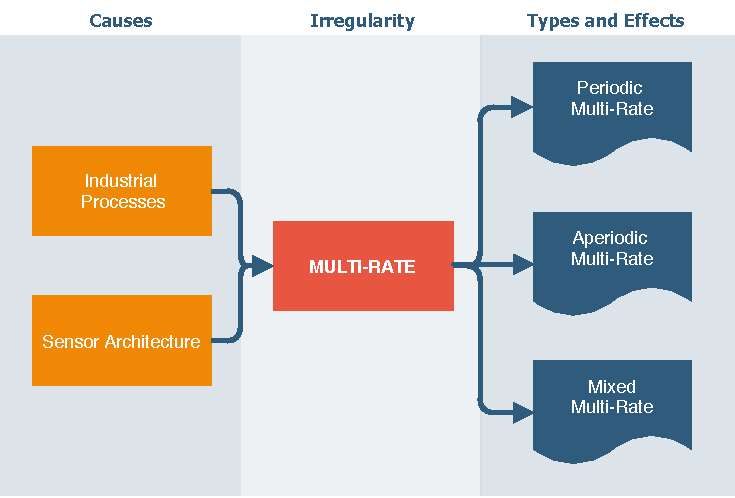
\includegraphics[width=0.75\textwidth]{Imagens/scheme_multi-rate.pdf}
	\caption[Multi-rate sampling diagram]{Multi-rate sampling diagram, showing the main causes (in orange) and types (in dark blue) of multi-rate sampling.}
	\label{fig:multi_rate}
\end{figure}

Many industrial processes need to control variables that can be measured by online instruments that provide regular, fast rate and delay free information, but with low precision. Therefore, more accurate data are needed and usually available after slow, irregular and human-dependent laboratory analysis \citep{Penarrocha2012, Fatehi2017}. The combination of both sources of measurements leads to a multi-rate sampling scenario. 

A more common approach is the use of various sensors measuring the same physical information, to obtain better estimates, which has been drawing attention from real world applications, such as target tracking, robotics, surveillance and military. For such strategy, the sampling rates perceived by the estimator are often different from one another. The work of \citep{Lin2016} and the references therein provide a wide coverage of scenarios derived from multi-sensor multi-rate systems. 

Figure \ref{fig:multi-rate} illustrates the ways multi-rate sampling can be manifested in a system. The different rates from the various sensor devices can be periodic (a), aperiodic (b) or even a mixture of both, as it is the case for most industrial applications with laboratory analysis.

\begin{figure}[!htb]
	\centering
	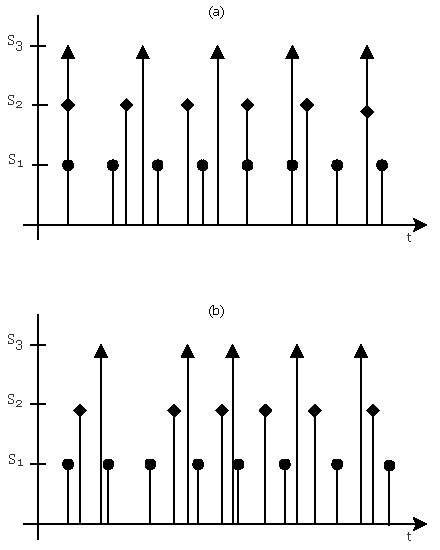
\includegraphics[width=0.5\textwidth]{Imagens/multi_rate.pdf}	
	\caption[Periodic and aperiodic multi-rate sampling scheme]{(a) Periodic and (b) aperiodic multi-rate sampling scheme. Labels $S_1$, $S_2$, $S_3$ refer to the sampling instants of three different sensors, from the highest sampling rate to the lowest sampling rate.}
	\label{fig:multi-rate}
\end{figure}

Aperiodic sampling rates can be described the same way as in Section \ref{sec:aperiodic}. Periodic multi-rate measurements can be modeled as

\begin{equation}
	y_i(k_iT_i) = z(k_iT_i) + v_i(k_iT_i)
\end{equation}

\noindent
where $y_i(k_iT_i)$ represents the $k_i^{th}$ observation from sensor $i$ with periodic sampling rate $T_i$ and $z(k_iT_i)$ is the $k$-th transmitted measurement of the $i$-th sensor.

\section{Time Synchronization}\label{sec:sync}

There are techniques to handle all the irregularities discussed in this chapter and still achieve efficient state estimation performance. Provided that the estimator is able to use the information on the time that measurements were taken, there are many algorithms that provide interesting results. 

In general, multi-sensor data fusion techniques for state estimation require that exact measurement timestamps are available in order to assimilate data properly \citep{Ping2003, Brahmi2013}. However, that is not always the case and situations may arise in which timestamps were not collected or their values are unreliable. Examples of the latter may occur when measurements are time stamped when they are received by the estimator instead of being time stamped at the moment it was taken, or when they are time stamped using temporal information from local clocks without centralized synchronization \citep{Julier2005}. 

In many practical applications, if sampling irregularity cannot be accounted for accordingly, data are fused using the time of arrival as timestamp \citep{Huck2011}, or irregularities such as OOSM are just disregarded completely \citep{Kwok2004}. The effects of such neglect has seldom been investigated, however. In one of the few studies, \citep{Julier2005} considered the state estimation problem for delayed but periodic observations with imprecise and unknown timestamps, with the assumption that they could be statistically characterized. They proposed an implementation of the covariance union (CU) technique, using the timestamp statistics in the filter update step. First, the method calculates the updates considering both the maximum and minimum expected delayed and then merged both results with a convex combination designed to minimize the state covariance matrix. CU algorithm was tested for the problem of estimating the states of a linear system, considering a random time delay, uniformly distributed between 2 and 10 time steps. Estimation performance was tested against four other methods: \textit{known delay}, that considers the time delay to be known perfectly, as a baseline for comparison; \textit{mean delay}, that assumes the delay to be always an average of 6 time steps; maximum likelihood, that calculates the likelihood of each possible time step and selects the highest; and Probabilistic Data Association Filter (PDAF) \citep{Bar-shalom2009}, that also calculates the likelihood of each step and averages the results using the likelihood as weight. They used the normalized state estimation error (NEES) test for consistency assessment, which we explain later in Section~\ref{sec:metrics}, for a linear system with two states. Therefore, the expected value of NEES for a consistent filter should be 2. The results are replicated in Table~\ref{tab:cu_consistency} for all algorithms. 

\begin{table}[!ht]
	\centering
	\setlength{\tabcolsep}{12pt}
	\caption[Consistency test results for fusion of time delayed measurements with uncertain timestamps]{Comparison of NEES consistency test results for fusion of time delayed measurements with uncertain timestamps for a linear system with two states}
	\renewcommand{\arraystretch}{1.5}
	\begin{tabular}{l  c }
		\toprule
		Method				& E$\left[\textrm{NEES}\right]$  \\
		\midrule
		Known delay 		& 1.9992  \\
		Mean delay 			& 37.6949  \\
		Max likelihood 		& 54.9323 \\
		Covariance union 	& 1.3172 \\
		PDAF & 1.8749 \\
		\bottomrule
	\end{tabular}
	\label{tab:cu_consistency}
\end{table}

As expected, the method with known delay was the most consistent, that is with $E\left[ \textrm{NEES} \right]$ results closer to 2. CU and PDAF were both consistent, with slightly overestimated state error. They argued that, although PDAF obtained better consistency results, it has significantly higher computational costs. Nevertheless, the results of the mean delay and maximum likelihood are highly inconsistent, showing that the neglect or oversimplification of the imprecision in timestamp leads to considerable performance degradation.

Another approach to overcome unknown timestamps on the presence of sampling irregularities was studied by \citep{Kwok2004}. In the presence of OOSM, when sensor information is sampled at much faster rates than filter update rates, the real-time particle filter (RTPF) proposed by them makes efficient use of all sensor information, instead of discarding sensor readings. That is achieved by dividing the received measurements among sample sets and then representing the states as a mixture of those sets.

Alternatively, in order to avoid performance degradation, one can make use of time synchronization schemes, widely used in communication networks, to ensure global time stamps. Wireless sensor networks (WSN) are particularly dependent on such techniques, due to limited computation, energy and communication resources of the sensing devices used. The works of \citep{Sivrikaya2004} and \citep{Roemer2003} provide detailed reviews on the time synchronization problem in sensor networks. 

%They explain the problem through computer clock mechanism. 
%
%With the aid of a hardware oscillator, local clocks from a sensing device node $i$ approximates real time $t$ as $C_i(t)$ by
%	
%\begin{equation}\label{eq:clock1}
%C_i(t) = a_it+b_i
%\end{equation}
%
%\noindent
%where $a_i(t)$ is the clock \textit{drift}, that is the clock frequency, and $b_i(t)$ represents an \textit{offset} value, or the difference from real value $t$.
%
%Clock approximations from two nodes in a network are compared by
%
%\begin{equation}\label{eq:clock2}
%C_1(t) = a_{12}C_2(t)+b_{12}
%\end{equation}
%
%\noindent
%where $a_{12}$ is the relative \textit{drift} and $b_{12}$ is the relative offset between nodes. 
%
%Under equations (\ref{eq:clock1}) and (\ref{eq:clock2}), the synchronization problem becomes the equalization of the computer clocks from all different $n$ devices, in its most strict form. Thus, synchronization strategies can either match all clock frequencies and offsets once or perform repeated offset corrections over time. There are more relaxed versions of synchronizations, such as the one proposed by \cite{Roemer2003}, that aims at maintaining only the order of events.	

Probably the most popular time synchronization method is the one being used in the internet environment for years, the Network Time Protocol (NTP), designed by \citep{Mills1991}. For most control and WNS applications, however, it is not suitable, due to very different requirements, such as energy consumption, precision and scalability \citep{Ganeriwal2003}. 

Another easy solution would be to equip all sensing devices in the network with a global positioning system (GPS) for a global time synchronization, but such solution is very expensive, not energy efficient and its signal might not work properly in every environment.

Therefore, many alternative methods have been proposed, and the work of \citep{Kaur2015} updates the studies from \citep{Sivrikaya2004}, with an exploration of the most recent synchronization protocols for sensor networks, that is: reference broadcast synchronization (RBS) \citep{Elson2002}; timing-sync protocol for sensor networks (TPSN) \citep{Ganeriwal2003};  delay measurement time synchronization (DMTS) \citep{Ping2003}; lightweight tree-based synchronization (LTS) \citep{Greunen2003}; tiny-sync mini-sync \citep{Sichitiu2003}; flooding time synchronization protocol (FTSP) \citep{Maroti2004}; lightweight and energy efficient time synchronization (LEETS) \citep{MingxiaXu2005}; time diffusion protocol (TDP) \citep{Su2005}; and time synchronization based on spanning tree (TSST) \citep{He2008}. A comparison adapted from Kaur ad Abhilasha is presented in Table~\ref{tab:sync}.


\begin{table}[!htb]
	\renewcommand{\arraystretch}{1.3}
	\caption[Comparison of time synchronization methods]{Comparison of time synchronization methods. Parameters are \textit{Precision, Energy Efficiency ($E.E.$) and Complexity ($Comp.$)}. Adapted from \citep{Kaur2015}}
	\label{tab:sync}
	\centering
	\begin{flushleft}
		
		{
			\footnotesize
			\begin{tabularx}{\linewidth}{
					>{\hsize=0.45\hsize}X
					>{\hsize=1.475\hsize}X
					>{\hsize=1.475\hsize}X
					>{\hsize=0.6\hsize}X}
				\hline
				\textbf{Protocol} 			& \textbf{Advantages}    			&  \textbf{Limitations} 		& \textbf{Parameters}\\ 
				\hline
				RBS & Eliminates random delays on the sender side & High amount of message exchanges and low transmission range & 29.1 $\mu s$ \ \ \ High $E.E.$ High $Comp.$ \\ \\
					
				TPSN & Eliminates the access, byte alignment and propagation times  & Does not estimate the clock drift; does not handle dynamic topology changes and demands high communication load & 16.9 $\mu s$ \ \ \ High $E.E.$ Low $Comp.$ \\ \\

				DMTS & Reduces the number of message exchanges  & Restricted to low resolution and low frequency external clocks & 32 $\mu s$ \ \ \ \ \ \ \ \ \ \ \ \ V. High $E.E.$ Low $Comp.$ \\ \\
					
				LTS & Robust and works well in the presence of dynamic links and fading.  & The accuracy of synchronization decreases linearly in the depth of the synchronization tree & Unknown \ \ \ Low $E.E.$ Low $Comp.$ \\ \\
									
				Tiny-Sync Mini-Sync & Tolerant to message losses and adequate for networks with limited bandwidth and computational power & Unsuited for mobile sensor networks, high convergence time, not scalable and little robustness & 945 $\mu s$ \ \ \ \ \ \ High $E.E.$ Low $Comp.$ \\ \\		
									
				FTSP & Robust, handles dynamic topology changes well and eliminates maximum delay components  & Does not eliminate propagation delay and is not scalable & 1.48 $\mu s$ \ \ \ High $E.E.$ High $Comp.$ \\ \\
										
				LEETS & Low power consumption and low amount of message exchanges & Requires a GPS receiver in the root node & 30 $\mu s$ \ \ \ \ \ \ \ 	High $E.E.$ Low $Comp.$ \\ \\
				
				TDP & Tolerant to message losses, high mobility and performs well even without external servers  & Very high convergence time & 100 $\mu s$ \ \ \ \ \ \ 	High $E.E.$ High $Comp.$ \\ \\
									
				TSST & Low synchronization error & Not scalable & Unknown  \ \ \ Low $E.E.$ Low $Comp.$ \\ \\
				
			\end{tabularx}
		}
	\end{flushleft}
\end{table}


\section{Chapter Summary and Final Remarks}

In this chapter, the main sampling irregularities are reviewed: time delay, packet loss, uncertain observation, aperiodic and multi-rate. Diagrams describing their causes, types and effects are shown for each of them. We also describe the necessary modifications to the observation models of state estimation algorithms. Most of the methods proposed in the literature to handle sampling irregularities rely on the correct time stamping of observations. Thus, time synchronization in sensor networks becomes crucial and its further explored. The most recent protocols developed to ensure a global time scale from sensing devices in large sensor networks are shown and compared.

However, the use of any time synchronization method requires computational, energy and resource consumption to some extent, apart from complex algorithms implementations. For sensor fusion performance applications in state estimation of sampled-data systems with irregular sampling, the investment might not be worth it. Thus, the next chapters try to shed some light in the evaluation of performance degradation in state estimation in the presence of irregular sampling, if timestamps are not available.


\clearpage
\afterpage{\blankpage}
%%%

% Demais Capítulos . . .
%==================================================================================================


%==================================================================================================
%                                       REFERÊNCIAS
%==================================================================================================
%!!!!!!!!!!!!!!!!!!!!!!!!!!!!!!!!!!!!!!!     ATENÇÃO     !!!!!!!!!!!!!!!!!!!!!!!!!!!!!!!!!!!!!!!!!!!
%	Para saber o número da primeira página das referencias, verifique o número da última página
% colocado no último capítulo (neste caso capítulo 3): arquivo pre.tex. Lembrando que cada capítulo 
% se inicia em ímpar.
%!!!!!!!!!!!!!!!!!!!!!!!!!!!!!!!!!!!!!!!!!!!!!!!!!!!!!!!!!!!!!!!!!!!!!!!!!!!!!!!!!!!!!!!!!!!!!!!!!!!
%%% Força a contagem da página.
\clearpage
\setcounter{page}{7}
%%%
\phantomsection
\addcontentsline{toc}{chapter}{Referências}

\DeclareRobustCommand{\refname}{\begin{center} Referências \end{center} \vspace*{2.cm}}
\bibliographystyle{bibformtese}          %   Arquivo que formata as referências (não modificar)

\bibliography{referencias}
%==================================================================================================


%==================================================================================================
%                                            ANEXO
%==================================================================================================
%!!!!!!!!!!!!!!!!!!!!!!!!!!!!!!!!!!!!!!!     ATENÇÃO     !!!!!!!!!!!!!!!!!!!!!!!!!!!!!!!!!!!!!!!!!!!
%	Para saber o número da primeira página do ANEXO, verifique o número da última página
% colocado nas REFERÊNCIAS. Lembrando que cada capítulo se inicia em ímpar.
%!!!!!!!!!!!!!!!!!!!!!!!!!!!!!!!!!!!!!!!!!!!!!!!!!!!!!!!!!!!!!!!!!!!!!!!!!!!!!!!!!!!!!!!!!!!!!!!!!!!
%%% Força a contagem da página.
\clearpage
\setcounter{page}{9}
%%%
\let\originalanexo=\anexo
% \def\anexo{\cleardoublepage\originalanexo}
\renewcommand*{\theHsection}{\thepart.\thesection}

\setcounter{chapter}{0}
\def\thechapter{\Alph{chapter}}

\phantomsection
\addcontentsline{toc}{chapter}{ANEXOS}
%%% Anexo A
% \begin{center}\label{ArquivosEntrada}
% \chapter{Arquivos de Entrada do $hp^2$FEM}
% \end{center}

\begin{center}
\anexo{-- \ \ Arquivos de Entrada do $hp^2$FEM}\label{AnexoA}
\end{center}

Os dados apresentados a seguir correspondem os arquivos de entrada utilizados para testar o problema
de projeção para quatro elementos quadrados.

\section{Arquivo .fem}\label{AnexoA:fem}

O arquivo a seguir apresenta as configurações para uma malha estruturada.

{\footnotesize
\begin{verbatim}
*TITLE
Title
*

*ELEMENT_GROUPS
1
1   4   SQUARE  1   4

*INCIDENCES
1 1 2 5 4
2 2 3 6 5
3 4 5 8 7
4 5 6 9 8

*DIMENSION
2

*COORDINATES
9
1   0   0
2   1   0
3   2   0
4   0   1
5   1   1
6   2   1
7   0   2
8   1   2
9   2   2

*GM_KEYPOINT
0

*GM_LINE
0 0

*GM_SURFACE
0 0

*GM_VOLUME
0 0

*END
#
# Developed by Gilberto Luis Valente da Costa
# e-mail: betogil@gmail.com
\end{verbatim}
}

\clearpage

\section{Arquivo .def}\label{AnexoA:def}

O arquivo a seguir apresenta as configurações para uma malha uniforme e p-uniforme.


{{\footnotesize
\begin{verbatim}
*POST_PROCESSOR
4 GID

*SOLUTION_DIRECTIVES
*SOLVER_TYPE
ELEMENT_ELEMENT

*ANALYSIS_TYPE
PROJECTION  CONSIST

*SOLUTION_ALGORITHM
LINEAR_SOLUTION

*LINEAR_SOLUTION_METHOD
GAUSS

*OPERATOR_TYPE
SYMMETRIC

*THEORETICAL_SOLUTION
L2 1 1 P s exp(3.1416*X)*sin((3.1416/4)*Y)*((X-1)^2)*(Y^2)


*GROUP_PARAMETERS_1

*MESH_TYPE_1
UNIFORM pUNIFORM

*SOLUTION_ORDER_1
4

*DOFS_GROUP_1
1 P 0 1 P 2 QX QY 0 0 0

*MATERIAL_1
HOOKE 2100 0.3 1.0E-06 1

*GEOMETRIC_PROPERTIES_1
1 1 1

*MAPPING_1
ISOPARAMETRIC

*KINEMATICS_1
INFINITE MATERIAL TOTAL_LAGRANGIAN

*PROBLEM_PARAMETERS_1
POISSON D1_MATRICES CONSIST CONSISTENT

*INTERPOLATION_1
STAND NODAL NON_HIERARCHICAL STANDARDLAGRANGE

*COLLOCATION_POINTS_1
EQUALLY_SPACED

*INTEGRATION_POINTS_1
GAUSS_LEGENDRE 2

*DOF
1
P
0
1
P
2
QX QY
0
0
0

*HOMOGENEOUS_DIRICHLET_BC
*HDBC_NODES
0
*HDBC_EDGES
0
*HDBC_FACES
0
*HDBC_KEYPOINTS
0
*HDBC_LINES
0
*HDBC_SURFACES
0

*NON_HOMOGENEOUS_DIRICHLET_BC
*NHDBC_NODES
0
*NHDBC_EDGES
0
*NHDBC_FACES
0
*NHDBC_KEYPOINTS
0
*NHDBC_LINES
0
*NHDBC_SURFACES
0


*LOAD_SETS
1

*LOAD_SET_1

*NODAL_LOADS_1
0
*KEYPOINT_LOADS_1
0
*EDGE_LOADS_1
0
*LINE_LOADS_1
0
*FACE_LOADS_1
0
*SURFACE_LOADS_1
0
*BODY_LOADS_1
4
1 1 P s exp(3.1416*X)*sin((3.1416/4)*Y)*((X-1)^2)*(Y^2)
2 1 P s exp(3.1416*X)*sin((3.1416/4)*Y)*((X-1)^2)*(Y^2)
3 1 P s exp(3.1416*X)*sin((3.1416/4)*Y)*((X-1)^2)*(Y^2)
4 1 P s exp(3.1416*X)*sin((3.1416/4)*Y)*((X-1)^2)*(Y^2)
*VOLUME_LOADS_1
0
*EDGE_PRESSURE_1
0
*FACE_PRESSURE_1
0
*LINE_PRESSURE_1
0
*SURFACE_PRESSURE_1
0

*END
#
# Developed by Gilberto Luis Valente da Costa
# e-mail: betogil@gmail.com
\end{verbatim}
}
%%%
%==================================================================================================


%==================================================================================================
%                                           APÊNDICE
%==================================================================================================
%!!!!!!!!!!!!!!!!!!!!!!!!!!!!!!!!!!!!!!!     ATENÇÃO     !!!!!!!!!!!!!!!!!!!!!!!!!!!!!!!!!!!!!!!!!!!
%	Para saber o número da primeira página do APENDICE, verifique o número da última página
% colocado nos ANEXOS. Lembrando que cada capítulo se inicia em ímpar.
%!!!!!!!!!!!!!!!!!!!!!!!!!!!!!!!!!!!!!!!!!!!!!!!!!!!!!!!!!!!!!!!!!!!!!!!!!!!!!!!!!!!!!!!!!!!!!!!!!!!
%%% Força a contagem da página.
\clearpage
\setcounter{page}{15}
%%%
\let\originalappendix=\appendix
% \def\appendix{\cleardoublepage\originalappendix}

\setcounter{chapter}{0}
\def\thechapter{\Alph{chapter}}

\phantomsection
\addcontentsline{toc}{chapter}{APÊNDICES}
%%% Apêndice A
\begin{center}
\appendix{-- \ \ Arquivos do analisador simbólico-numérico}\label{ApendiceA}
\end{center}



\section{Arquivo do analisador léxico}\label{ApendiceA:Lex}

\lstinputlisting[language=Perl, label=sources:AnalisadorLexico, caption={Arquivo para geração de
um analisador léxico}]{./apendices/sources/calculator.l}


\section{Arquivo do analisador sintático}\label{ApendiceA:Sintatico}

\lstinputlisting[language=Perl, label=sources:AnalisadorSintatico, caption={Arquivo para geração de
um analisador sintático}]{./apendices/sources/calculator.y}


\section{Arquivo de interface entre o $hp^2$FEM e o analisador
simbólico-numérico}\label{ApendiceA:Analisador}

\lstinputlisting[language=Perl, label=sources:AnalisadorSintatico, caption={Arquivo de interface
entre o \textit{software} $hp^2$FEM e o analisador
simbólico-numérico}]{./apendices/sources/calculator.y}



% Apêndices\index{apêndices} complementam o texto principal da tese com informações para leitores com
% especial interesse no tema, devendo ser considerados leitura opcional, ou seja, o entendimento do
% texto principal da tese não deve exigir a leitura atenta dos apêndices.
% 
% Apêndices usualmente contemplam provas de teoremas, deduções de fórmulas\index{fórmulas}
% matemáticas\index{fórmulas!matemáticas}, diagramas esquemáticos, gráficos e trechos de código.
% Quanto a este último, código extenso não deve fazer parte da tese, mesmo como apêndice. O ideal é
% disponibilizar o código na Internet para os interessados em examiná-lo ou utilizá-lo.
% 
% \section{Seção do apêndice}
% Equação:
% \begin{equation}\label{eq:WTS}
% w_i=X_{1}^i(x_1)t \ldots tX_{n}^i(x_n)
% \end{equation}
     % Usando input fez o "APÊNDICES" apareçer no lugar certo no sumario
%%%
%==================================================================================================


% %==================================================================================================
% %                                        ÍNCICE REMISSIVO
% %==================================================================================================
% \cleardoublepage
% \phantomsection
% \addcontentsline{toc}{chapter}{ÍNDICE}
% \renewcommand{\indexname}
% {\begin{center} {\large ÍNDICE} \end{center}}
% \printindex
% % Apêndice(s)
% %\appendix


%===============================================================================
% Apendice A

\chapter{Apendice A}\label{apendA}

%===============================================================================



%  %==================================================================================================

% Fim do texto
\end{document}
